\pdfbookmark{Общая характеристика работы}{characteristic}             % Закладка pdf

\setcounter{page}{1}

\begin{center}
\section*{Общая характеристика работы}
\end{center}

\newcommand{\actuality}{\pdfbookmark[1]{Актуальность}{actuality}\textbf{\actualityTXT}}
\newcommand{\progress}{\pdfbookmark[1]{Разработанность темы}{progress}\textbf{\progressTXT}}
\newcommand{\aim}{\pdfbookmark[1]{Цели}{aim}{\textbf\aimTXT}}
\newcommand{\tasks}{\pdfbookmark[1]{Задачи}{tasks}\textbf{\tasksTXT}}
\newcommand{\aimtasks}{\pdfbookmark[1]{Цели и задачи}{aimtasks}\aimtasksTXT}
\newcommand{\novelty}{\pdfbookmark[1]{Научная новизна}{novelty}\textbf{\noveltyTXT}}
\newcommand{\influence}{\pdfbookmark[1]{Практическая значимость}{influence}\textbf{\influenceTXT}}
\newcommand{\methods}{\pdfbookmark[1]{Методология и методы исследования}{methods}\textbf{\methodsTXT}}
\newcommand{\defpositions}{\pdfbookmark[1]{Положения, выносимые на защиту}{defpositions}\textbf{\defpositionsTXT}}
\newcommand{\reliability}{\pdfbookmark[1]{Достоверность}{reliability}\textbf{\reliabilityTXT}}
\newcommand{\probation}{\pdfbookmark[1]{Апробация}{probation}\textbf{\probationTXT}}
\newcommand{\contribution}{\pdfbookmark[1]{Личный вклад}{contribution}\textbf{\contributionTXT}}
\newcommand{\publications}{\pdfbookmark[1]{Публикации}{publications}\textbf{\publicationsTXT}}


{\actuality}
Задачи термоупругости очень популярны в различных инженерных приложениях, так как температурные деформации могут существенным образом повлиять на функциональные свойста рассматриваемых объектов, вплоть до их полного выхода из строя. Особенно популярны такого рода задачи в аэрокосмической отрасли при моделировании поведения обшивок корпусов и двигателей летательных аппаратов \cite{Aerocosmos1, Aerocosmos2, Aerocosmos3}, так как они подвергаются очень высоким и в то же время неравномерным нагружениям \cite{Aerocosmos4, Aerocosmos5, Aerocosmos6, Aerocosmos7}. Помимо аэрокосмической отрасли такие задачи могут быть востребованы в строительстве, особенно в строительстве критической инфраструктуры, такой, например, как атомные электространции \cite{StroyMech1, StroyMech2}. Однако и гражданская инфраструктура подвергается анализу влияния таких разрушительных явлений как пожары \cite{StroyMech3, StroyMech4} или обычная циклическая смена сезона \cite{StroyMech5, StroyMech6} при воздействии которых конструкция не должна потерять устойчивость. В микроэлектронике эти задачи также не остаются без внимания \cite{MicroElectronic1, MicroElectronic2}, а учитывая возрастающее количество вычислительных мощностей и популярность носимой электроники возникают задачи об эффективном отводе тепловой энергии \cite{MicroElectronic3}.

Все перечисленные ранее и многие другие задачи объединяет потребность в создании новых материалов, которые будут отвечать соответствующим их использованию требованиям. На сегодняшний день, в некоторых отраслях требования к свойствам материалов становятся уже настолько высокими, что при их создании приходится учитывать структуру материала на микро- и наноуровне \cite{MaterialStructure1, MaterialStructure2, MaterialStructure3}, так как их свойства могут напрямую зависеть от молекулярной структуры. Такие материалы принято называть структурно-чувствительными материалами, а создание материалов с наперёд заданными свойствами на сегодняшний момент является одной из сложнейших, но вместе с этим крайне актуальной областью материаловедения \cite{Auxetics}.

Помимо проблемы создания структурно-чувствительных материалов многие исследователи также сталкиваются с проблемой моделирования их поведения. При рассмотрении наномасштабных структур пропадает возможность использовать гипотезу сплошности среды из-за чего классические модели механики сплошной среды не могут даже на качественном уровне передать все особенности их поведения. Преобладание таких эффектов как микровращения отдельных зёрен материала, микродислокации, различные дальнодействующие и многие другие масштабные эффекты могут быть смоделированы только при помощи новых математических моделей.

К счастью, на сегодняшний день существует большое количество моделей способных описать различные масштабные эффекты, однако, способы моделирования могут достаточно сильно различаться между собой при рассмотрении разных линейных размеров и временных отрезков. Таким образом возникают иерархии моделей способных качественно и количественно описать различные аспекты поведения материала на разных масштабах. Это в свою очередь приводит к идее многомасштабного моделирования \cite{Multiscale1}, где, например, некоторые характеристики материала можно вычислять при помощи моделей находящихся ниже по иерархии и передавать полученные в расчётах параметры в вышестоящие модели.

Для механики твёрдого тела одна из возможных иерархий моделей проиллюстрирована на рис. \ref{fig:ModelsHierarchy}. Согласно такому представлению, модели использующие аппарат квантовой механики \cite{QuantumModelling1, QuantumModelling2} находятся на первой ступени иерархии, а их применение ограничено масштабами сопоставимыми с ядрами атомов и их молекулярных соединений, то есть в диапазоне от нескольких ангстрем до нескольких нанометров. На второй ступене иерархии находятся модели молекулярной динамики \cite{MD1, MD2, MD3, MD4}, такие модели могут описывать поведение сложных соединений, например, больших полимерных молекул и прочих наномасштабных объектов, размеры которых не превосходят нескольких десятков нанометров. На третьей ступене располагаются статистические модели, в частности модели в основе которых лежит метод Монте-Карло \cite{MonteCarlo1, MonteCarlo2}. В таких моделях расчёты проводятся многократно, а структура рассматриваемого объекта генерируется случайным образом по особым правилам после чего полученные таким способом результаты осредняют или вычисляют на их основе вероятностные характеристики материала. И на последней --- четвёртой ступени иерархии стоят континуальные модели, в частности модели механики сплошной среды \cite{MSS}. Такие модели оперируют гипотезой сплошностью среды и абсолютности времени, то есть не учитывают дискретность рассматриваемого вещества.

\begin{figure}[ht]
    \centerfloat{
        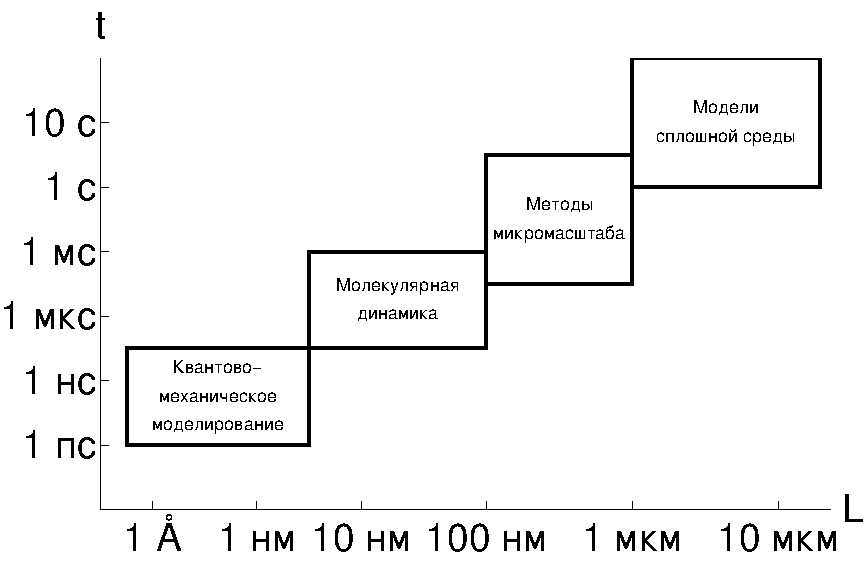
\includegraphics[width=0.85\textwidth]{pics/ModelsHierarchy.pdf}
    }
    \caption{Иерархия моделей.}\label{fig:ModelsHierarchy}
\end{figure}

Однако, несмотря на то, что модели молекулярной динамики и статистические модели находятся на более низких ступенях иерархии, чем модели сплошной среды, анализ объектов при помощи этих моделей без численных экспериментов крайне ограничен \cite{MDExperiment}. Поэтому с середины XX века набирают популярность модели обобщённой механики сплошной среды, которые распространяют применение моделей высшего уровня на области применения моделей низшего уровня. Одна из первых таких моделей была предложена в работе братьев Эжен и Франсуа Коссера \cite{Cosserat}, где помимо трансляционных степеней свободы также учитывались и вращательные компоненты движения, которые связаны с трансляционными рядом соотношений из-за чего тензор напряжений становится нессиметричным. Позже, спустя пол века, эта теория была связана с теорией дислокаций в работе V.~G{\"u}nther \cite{CosseratAndDislocation} и дополнена законом сохранения микроинерции в работе A.C.~Eringen \cite{Eringen2, Eringen3} в связи с чем теорию начали называть микрополярной теорией упругости. Также к работам связанным с исследованием микрополярной теории упругости можно отнести работы R.D.~Mindlin \cite{Mindlin1, Mindlin2, Mindlin3}, и работы D.B.~Bogy \cite{Bogy} и Y.C.~Hsu \cite{Hsu}, в которых авторы рассматривали применение этой теории к задачам с концентраторами возникающим в углах и отверстиях соответсвенно. В это же время теория приобрела своё развитие в работах советских учёных Э.Л.~Аэро и Е.В.~Кувшинского \cite{Aero1,Aero2}, а также была рассмотрена в работах Н.Ф.~Морозова \cite{Morozov} и Г.Н. Савина \cite{Savin}.

Дальнейшее развитие микрополярной теории упругости привело к появлению микроморфных моделей \cite{Eringen4, Micromorph1, Micromorph2}, в которые помимо вращательных компонент движения могут быть включены дополнительные переменные связанные с деформацией материала, при этом микрополярная теория упругости ялвяется лишь частным случаем микроморфных моделей. К сожалению, использование таких моделей сопряжено с трудностью определения материальных коэффициентов, которых в такого рода моделях становится достаточно много.

Список рассмотренных моментных моделей, а также авторов, которые занимались их развитием и исследованием далеко не исчерпывающий, однако, стоит также уделить внимание другому классу моделей обобщённой механики сплошной среды учитывающих дальнодействующие эффекты. Это градиентные и нелокальные модели, которые также получили своё развитие в 60-х годах XX века. Первые модели градиентной теории упругости были сформулированы в работах Toupin~R.A. \cite{Toupin} и Mindlin~R.D. \cite{Mindlin4, Mindlin5}, которые сейчас в литературе принято называть моделями Миндлина --- Тупина \cite{ToupinMindlin1, ToupinMindlin2, ToupinMindlin3}. Позже в работе G.~Ahmadi и K.~Firoozbakhsh \cite{GradientThermoelasticity} эти модели получили связь с температурными деформациями. Но как и микроморфные модели градиентные модели обладают тем же недостатком --- большое количество материальных констант, которые необходимо определить, поэтому в 90-х годах XX века в работах E.C.~Aifantis и его соавторов \cite{Aifantis1, Aifantis2} была рассмотренна упрощёная модель градиентной теории упругости, в которой напряжения зависят от деформации и её второго градиента, а также введён всего один дополнительный материальный параметр внутренней длины.

Нелокальные модели в отличие от градиентных оперируют интегральными выражениями типа свёртки. Впервые описание таких моделей было представлено в работе E.~Kr{\"o}ner \cite{Kroner}, где рассматривались упругие среды с дальнодействующими силами сцепления. Модели нелокальной упругости в термодинамическом контексте были рассмотрены в работах D.G.B.~Edelen, A.E.~Green и N.~Laws \cite{Edelen1, Edelen2}, позже к работе присоединился и A.C.~Eringen \cite{Eringen5, Eringen6}. Исследование условий обеспечивающих существование фундаментнальных решений было проведено в работе D. Rogula \cite{Rogula1982}. Вопросы, связанные с существованием и единственностью решения нелокальной начально-краевых задач упругости были рассмотрены в работах S.B.~Altan \cite{Altan1, Altan2}, а также для задач нелокальной термоупругости \cite{Altan3, Altan4}. В дальнейшем A.C.~Eringen представит работу, в которой описан единый подход к построению нелокальных теорий для упругих тел в работе \cite{Eringen1}, в связи с чем в литературе нелокальные модели часто называют моделями Эрингена \cite{BondaryLayer, Tuna, Rahmani}.

Связь градиентной модели Айфантиса и нелокальной \cite{Aifantis3, Gao}.

Текущая работа посвящена исследованию нелокальных моделей, а точнее даже их модификации с добавлением регуляризационного слагаемого относящегося к классической или локальной теории. Такой подход был предложен в работе Polizzoto \cite{Polizzotto1}.

\cite{SaintVenant}.

Поиск решений интегро-дифференциальных уравнений представляет из себя достаточно сложную задачу. В этом случае необходимо прибегать к использованию различных численных методов, специально адаптированных под данный класс уравнений. В этом направлении есть уже достаточно большое количество работ, предлагающие использовать различные методы решения. Наиболее общим и популярным является метод конечных элементов (FEM), который применительно к данному классу уравнений иногда ещё называют методом нелокальных конечных элементов (NL-FEM) \cite{Polizzotto2, Pisano1}. Однако его использование сопряжёно с большой вычислительной сложностью, поэтому некоторые ииследователи прибегают к возможностям интегральных преобразований откуда был получен метод на основе быстрого преобразования Гаусса (FEMFGT) \cite{FastGaussTransform}. К сожалению, использование этого метода сопряжено с рядом трудностей, так как для его применения необходима достаточно подробная сетка, чтобы избежать возможных осциляций решения, также сложность вызывает контроль точности получаемых решений. Помимо сеточных методов большой популярностью пользуются и бессеточные подходы на основе радиальных базисных функций \cite{RadialBasis}, безэлементный метод Галёркина (EFG) и метод конечных точек (FPM) \cite{MeshFree}. Также были предложены подходы с использованием пограничного слоя \cite{BondaryLayer} и на основе полиномов Чебышева \cite{ChebPolynom}.

В рамках этой работы было принято решение остановиться на методе конечных элементов, так как этот метод достаточно хорошо изучен и его относительно легко реализовать и модифицировать под рассматриваемый класс уравнений. Также этим методом легко решать задачи на областях со сложной геометрической формой, а большое количество редакторов и генераторов сеток упрощает процесс моделирования. Реализация данного метода включена в программный комплекс NonLocFEM, структуру которого мы рассмотрим в третьей главе диссертации.

%\ifsynopsis
%Этот абзац появляется только в~автореферате.
%\else
%Этот абзац появляется только в~диссертации.
%\fi

% {\progress}
% Этот раздел должен быть отдельным структурным элементом по
% ГОСТ, но он, как правило, включается в описание актуальности
% темы. Нужен он отдельным структурынм элемементом или нет ---
% смотрите другие диссертации вашего совета, скорее всего не нужен.

{\aim}
исследования является изучение особенностей рассматриваемых моделей термоупругости, а также сравнение решений полученных при их использовании с решениями полученными при использовании классических моделей механики сплошной среды.

Для достижения поставленной цели потребовалось решить {\tasks}:
\begin{enumerate}[beginpenalty=10000] % https://tex.stackexchange.com/a/476052/104425
  \item Разработка определяющих соотношений модели термоупругости нелокальной среды в интегро-дифференциальной форме..
  \item Разработка алгоритмов численного решения с их последующей оптизацией для более эффективного использования на многопроцессорных вычислительных машинах.
  \item Реализация полученных алгоритмов в виде программного комплекса.
  \item Исследование поведения модели на примере решения определённого ряда задач с известными решениями в классической постановке, сравнение получившихся решений и определение закономерностей.
\end{enumerate}


{\novelty}
\begin{enumerate}[beginpenalty=10000] % https://tex.stackexchange.com/a/476052/104425
  \item Разработаны эффективные методы решения на основе метода конечных элементов с обобщением на интегро-дифференциальные уравнения, которые обладают хорошей масштабируемостью и предназначены для вычислений на многопроцессорных вычислительных машинах с общей и распределённой памятью.
  \item Разработан программный комплекс NonLocFEM, в котором реализованы все представленные в работе алгоритмы и методы для моделирования поведения структруно-чувствительных материалов.
  \item Проведено качественное сравнение между результатами полученными с использованием классической и нелокальной теориями, которые свидетельствуют о снижении роли концентраторов в распределениях полей напряжений и плотности теплового потока.
  \item Исследованы границы спектров собственных чисел матриц и установлены связи между спектрами матриц ассемблированных в классической и нелокальной постановках.
\end{enumerate}

{\influence}
моделей рассмотренных в диссертации состоит в возможности описания поведения термомеханических состояний структурно-чувствительных материалов, параметры модели очевидным образом влияют на решения, что позволяет тонко настраивать модель при исследованиях. Разработанный программный комплекс дополняет рассматриваемую модель, позволяет проводить расчёты на произвольных областях со всеми рассматриваемыми в моделе параметрами, а благодаря открытому исходному код и модульной структуре существует возможность без труда вносить в него изменения и добавлять новые типы расчётов при модификации математической модели.

{\methods}
В диссертации используются как классические принципы механики деформируемого твёрдого тела, так и новые относящиеся к нелокальной теории термоупругости, а также численные методы в основе которых лежит метод конечных элементов.

{\defpositions}
\begin{enumerate}[beginpenalty=10000] % https://tex.stackexchange.com/a/476052/104425
 	\item Модель нелокальной термоупругости позволяющая описать процессы теплопроводности и напряжённо-деформированного состояния в структурно-чувствительных материалах.
	\item Численный алгоритм решения на основе метода конечных элементов, адапатированный под многопроцессорные вычислительные системы.
	\item Программный комплекс NonLocFEM, в рамках которого реализованы все рассматриваемые в работе методы решений.
\end{enumerate}

{\reliability} гарантирует строгость используемого математического аппарата, сравнение расчётов с известными теоретическими результатами и аналитическими решениям, а также результатами, полученными ранее другими авторами.


{\probation}
проводилась в обсуждениях на следующих конференциях:
\begin{enumerate}
	\item Международная научно-техническая конференция <<Актуальные проблемы прикладной математики, информатикии и механики>> (Воронеж, 2019, 2021);
	\item Международная конференция <<International Conference of Numerical Analysis and Applied Mathematics>> (Родос, Греция, 2021);
	\item Международная научная конференция <<Фундаментальные и Прикладные Задачи Механики>> (Москва, 2021);
	\item Всероссийская конференция по численным методам решения задач теории упругости и пластичности (Красноярск, 2023);
	\item Математическое моделирование, численные методы и инженерное программное обеспечение (Москва, 2023).
\end{enumerate}

{\contribution}
Все исследования, представленные в диссертационной работе, а также разработка программного комплекса выполнены лично соискателем в процессе научной деятельности. Из совместных публикаций в диссертацию включен лишь тот материал, который принадлежит соискателю, заимствованный материал обозначен в работе ссылками.

\ifnumequal{\value{bibliosel}}{0}
{%%% Встроенная реализация с загрузкой файла через движок bibtex8. (При желании, внутри можно использовать обычные ссылки, наподобие `\cite{vakbib1,vakbib2}`).
    {\publications} Основные результаты по теме диссертации изложены
    в~XX~печатных изданиях,
    X из которых изданы в журналах, рекомендованных ВАК,
    X "--- в тезисах докладов.
}%
{%%% Реализация пакетом biblatex через движок biber
    \begin{refsection}[bl-author, bl-registered]
        % Это refsection=1.
        % Процитированные здесь работы:
        %  * подсчитываются, для автоматического составления фразы "Основные результаты ..."
        %  * попадают в авторскую библиографию, при usefootcite==0 и стиле `\insertbiblioauthor` или `\insertbiblioauthorgrouped`
        %  * нумеруются там в зависимости от порядка команд `\printbibliography` в этом разделе.
        %  * при использовании `\insertbiblioauthorgrouped`, порядок команд `\printbibliography` в нём должен быть тем же (см. biblio/biblatex.tex)
        %
        % Невидимый библиографический список для подсчёта количества публикаций:
        \printbibliography[heading=nobibheading, section=1, env=countauthorvak,          keyword=biblioauthorvak]%
        \printbibliography[heading=nobibheading, section=1, env=countauthorwos,          keyword=biblioauthorwos]%
        \printbibliography[heading=nobibheading, section=1, env=countauthorscopus,       keyword=biblioauthorscopus]%
        \printbibliography[heading=nobibheading, section=1, env=countauthorconf,         keyword=biblioauthorconf]%
        \printbibliography[heading=nobibheading, section=1, env=countauthorother,        keyword=biblioauthorother]%
        \printbibliography[heading=nobibheading, section=1, env=countregistered,         keyword=biblioregistered]%
        \printbibliography[heading=nobibheading, section=1, env=countauthorpatent,       keyword=biblioauthorpatent]%
        \printbibliography[heading=nobibheading, section=1, env=countauthorprogram,      keyword=biblioauthorprogram]%
        \printbibliography[heading=nobibheading, section=1, env=countauthor,             keyword=biblioauthor]%
        \printbibliography[heading=nobibheading, section=1, env=countauthorvakscopuswos, filter=vakscopuswos]%
        \printbibliography[heading=nobibheading, section=1, env=countauthorscopuswos,    filter=scopuswos]%
        %
        \nocite{*}%
        %
        {\publications} Основные результаты по теме диссертации изложены в~\arabic{citeauthor}~печатных изданиях,
        \arabic{citeauthorvak} из которых изданы в журналах, рекомендованных ВАК\sloppy%
        \ifnum \value{citeauthorscopuswos}>0%
            , \arabic{citeauthorscopuswos} "--- в~периодических научных журналах, индексируемых Web of~Science и Scopus\sloppy%
        \fi%
        \ifnum \value{citeauthorconf}>0%
            , \arabic{citeauthorconf} "--- в~тезисах докладов.
        \else%
            .
        \fi%
        \ifnum \value{citeregistered}=1%
            \ifnum \value{citeauthorpatent}=1%
                Зарегистрирован \arabic{citeauthorpatent} патент.
            \fi%
            \ifnum \value{citeauthorprogram}=1%
                Зарегистрирована \arabic{citeauthorprogram} программа для ЭВМ.
            \fi%
        \fi%
        \ifnum \value{citeregistered}>1%
            Зарегистрированы\ %
            \ifnum \value{citeauthorpatent}>0%
            \formbytotal{citeauthorpatent}{патент}{}{а}{}\sloppy%
            \ifnum \value{citeauthorprogram}=0 . \else \ и~\fi%
            \fi%
            \ifnum \value{citeauthorprogram}>0%
            \formbytotal{citeauthorprogram}{программ}{а}{ы}{} для ЭВМ.
            \fi%
        \fi%
        % К публикациям, в которых излагаются основные научные результаты диссертации на соискание учёной
        % степени, в рецензируемых изданиях приравниваются патенты на изобретения, патенты (свидетельства) на
        % полезную модель, патенты на промышленный образец, патенты на селекционные достижения, свидетельства
        % на программу для электронных вычислительных машин, базу данных, топологию интегральных микросхем,
        % зарегистрированные в установленном порядке.(в ред. Постановления Правительства РФ от 21.04.2016 N 335)
    \end{refsection}%
    \begin{refsection}[bl-author, bl-registered]
        % Это refsection=2.
        % Процитированные здесь работы:
        %  * попадают в авторскую библиографию, при usefootcite==0 и стиле `\insertbiblioauthorimportant`.
        %  * ни на что не влияют в противном случае
        \nocite{vakbib2}%vak
        \nocite{patbib1}%patent
        \nocite{progbib1}%program
        \nocite{bib1}%other
        \nocite{confbib1}%conf
    \end{refsection}%
        %
        % Всё, что вне этих двух refsection, это refsection=0,
        %  * для диссертации - это нормальные ссылки, попадающие в обычную библиографию
        %  * для автореферата:
        %     * при usefootcite==0, ссылка корректно сработает только для источника из `external.bib`. Для своих работ --- напечатает "[0]" (и даже Warning не вылезет).
        %     * при usefootcite==1, ссылка сработает нормально. В авторской библиографии будут только процитированные в refsection=0 работы.
}

%При использовании пакета \verb!biblatex! будут подсчитаны все работы, добавленные
%в файл \verb!biblio/author.bib!. Для правильного подсчёта работ в~различных
%системах цитирования требуется использовать поля:
%\begin{itemize}
%        \item \texttt{authorvak} если публикация индексирована ВАК,
%        \item \texttt{authorscopus} если публикация индексирована Scopus,
%        \item \texttt{authorwos} если публикация индексирована Web of Science,
%        \item \texttt{authorconf} для докладов конференций,
%        \item \texttt{authorpatent} для патентов,
%        \item \texttt{authorprogram} для зарегистрированных программ для ЭВМ,
%        \item \texttt{authorother} для других публикаций.
%\end{itemize}
%Для подсчёта используются счётчики:
%\begin{itemize}
%        \item \texttt{citeauthorvak} для работ, индексируемых ВАК,
%        \item \texttt{citeauthorscopus} для работ, индексируемых Scopus,
%        \item \texttt{citeauthorwos} для работ, индексируемых Web of Science,
%        \item \texttt{citeauthorvakscopuswos} для работ, индексируемых одной из трёх баз,
%        \item \texttt{citeauthorscopuswos} для работ, индексируемых Scopus или Web of~Science,
%        \item \texttt{citeauthorconf} для докладов на конференциях,
%        \item \texttt{citeauthorother} для остальных работ,
%        \item \texttt{citeauthorpatent} для патентов,
%        \item \texttt{citeauthorprogram} для зарегистрированных программ для ЭВМ,
%        \item \texttt{citeauthor} для суммарного количества работ.
%\end{itemize}
% Счётчик \texttt{citeexternal} используется для подсчёта процитированных публикаций;
% \texttt{citeregistered} "--- для подсчёта суммарного количества патентов и программ для ЭВМ.

%Для добавления в список публикаций автора работ, которые не были процитированы в
%автореферате, требуется их~перечислить с использованием команды \verb!\nocite! в
%\verb!Synopsis/content.tex!.
 % Характеристика работы по структуре во введении и в автореферате не отличается (ГОСТ Р 7.0.11, пункты 5.3.1 и 9.2.1), потому её загружаем из одного и того же внешнего файла, предварительно задав форму выделения некоторым параметрам

%Диссертационная работа была выполнена при поддержке грантов \dots

%\underline{\textbf{Объем и структура работы.}} Диссертация состоит из~введения,
%четырех глав, заключения и~приложения. Полный объем диссертации
%\textbf{ХХХ}~страниц текста с~\textbf{ХХ}~рисунками и~5~таблицами. Список
%литературы содержит \textbf{ХХX}~наименование.

\pdfbookmark{Содержание работы}{description}                          % Закладка pdf
\begin{center}
\section*{Содержание работы}
\end{center}
\textbf{Во введениии} обоснована актуальность исследований, проводимых в рамках данной диссертационной работы, приведён обзор научной литературы, сформулированы цели исследования, поставлены задачи, а также изложена научная новизна и практическая значимость.

\textbf{Первая глава} посвящена описанию основных соотношений моделей нелокальной теплопроводности и термоупругости.

\underline{В разделе 1.1} представлен интегральный нелокальный оператор
\begin{gather}
	\label{eq:NonlocalOperator}
	\mathcal{N} [f(\boldsymbol{x})] = 
	p_1 f(\boldsymbol{x}) + 
	p_2 \int\limits_{S'(\boldsymbol{x}') \cap S} 
		\varphi(\boldsymbol{x}, \boldsymbol{x}') f(\boldsymbol{x}')
	dS'(\boldsymbol{x}'),
	\quad
	\boldsymbol{x}' \in S'(\boldsymbol{x}).
\end{gather}
Здесь $f(\boldsymbol{x})$ --- выражение, описывающее сохраняющуюся физическую субстанцию;
$p_1 > 0$ и $p_2 \geqslant 0$ --- весовые параметры модели такие, что $p_1 + p_2 = 1$;
$\varphi$~---~функция нелокального влияния, нормированная положительная монотонно убывающая функция в области $S'(\boldsymbol{x})$; 
$\boldsymbol{x}'$~--- точка в области $S'(\boldsymbol{x})$;
$S'(\boldsymbol{x})$ --- область нелокального влияния с центром в точке $\boldsymbol{x} \in S$;
$S$ --- область, занимаемая рассматриваемым телом.

\underline{В разделе 1.2} представлено описание уравнения стационарной теплопроводности
\begin{gather}
	\label{eq:StationaryHeatEquation}
	\nabla \cdot \boldsymbol{q} = q_V,
\end{gather}
где $q_V$ --- объёмная плотность мощности внутренних источников и стоков теплоты, а вектор плотности теплового потока $\boldsymbol{q}$ определён как обобщённый закон Био --- Фурье с использованием нелокального оператора (\ref{eq:NonlocalOperator})
\[
	\boldsymbol{q}(\boldsymbol{x}) = 
	\mathcal{N} \left( -\widehat{\boldsymbol{\lambda}} \cdot \nabla T \right).
\]
Здесь $\widehat{\boldsymbol{\lambda}}$ --- тензор теплопроводности;
$T = T (\boldsymbol{x})$ --- поле температуры.

\underline{В разделе 1.3} представлено описание уравнения равновесия
\begin{gather}
	\label{eq:EquilibriumEquation}
	-\nabla \cdot \widehat{\boldsymbol{\sigma}} = \boldsymbol{b},
\end{gather}
где $\boldsymbol{b}$ --- вектор плотности объёмных сил; тензор напряжений $\widehat{\boldsymbol{\sigma}}$, определён, как обобщённый закон Дюамеля --- Неймана с использованием нелокального оператора (\ref{eq:NonlocalOperator})
\[
	\widehat{\boldsymbol{\sigma}}(\boldsymbol{x}) =
	\mathcal{N} \left(
		\widehat{\text{\textbf{C}}} \cdot \cdot 
		\left( \widehat{\boldsymbol{\varepsilon}} - \widehat{\boldsymbol{\alpha}}^T \Delta T \right)
	\right),
\]
где $\widehat{\varepsilon} = (\boldsymbol{u} + (\nabla \boldsymbol{u})^T) / 2$ --- тензор деформации;
$\boldsymbol{u}$ --- вектор перемещений;
$\widehat{\text{\textbf{C}}}$ --- тензор коэффициентов упругости;
$\widehat{\boldsymbol{\alpha}}^T$ --- тензор температурных коэффициентов линейного расширения;
$\Delta T = T - T_0$ --- разница между текущим распределением температуры $T$ и распределением $T_0$, при котором отсутствуют температурные деформации.

\underline{В разделе 1.4} определены два семейства функций нелокального влияния $\varphi$: полиномиальное семейство функций на ограниченных областях нелокального влияния $S'(\boldsymbol{x})$
\begin{gather}
	\label{eq:Polynomial}
	\varphi_{p,q}^{P}(\boldsymbol{x}, \boldsymbol{x}') =
	\begin{cases}
		A(1 - \rho_n(\boldsymbol{x}, \boldsymbol{x}')^p)^q, \quad &\rho_n(\boldsymbol{x}, \boldsymbol{x}') \leqslant 1, \\
		0, &\rho_n(\boldsymbol{x}, \boldsymbol{x}') > 1,
	\end{cases}
\end{gather}
и экспоненциальное семейство функций на неограниченных областях нелокального влияния $S'(\boldsymbol{x})$
\begin{gather}
	\label{eq:Exponential}
	\varphi_{p,q}^{E} (\boldsymbol{x}, \boldsymbol{x}') =
	A \exp \left(-q\rho_n(\boldsymbol{x}, \boldsymbol{x}')^p \right).
\end{gather}
Параметры для обеих семейств функций имеют одинаковый смысл: $p$ и $q$~--- параметры плотности распределения; $A$ --- нормировочный множитель; $\rho_n(\boldsymbol{x}, \boldsymbol{x}')$ --- метрическая функция.

\textbf{Вторая глава} посвящена построению численных схем решения уравнений стационарной теплопроводности и равновесия. В основе численных схем использован метод конечных элементов.

\underline{В разделе 2.1} очень кратко изложены базовые соотношения метода конечных элементов: определено понятие конечного элемента, свойства базиса конечного элемента, способ перехода от локальной системы координат элемента к глобальной и применение конечных элементов для аппроксимации функций.

\underline{В разделе 2.2} описан способ аппроксимации уравнений стационарной теплопроводности (\ref{eq:StationaryHeatEquation}) и равновесия (\ref{eq:EquilibriumEquation}), а также приведена последовательность преобразований, после которых приходим к СЛАУ, соответствующим уравнению стационарной теплопроводности и уравнению равновесия
\begin{gather}
	\label{eq:ThermalSLAE}
	\left( p_1 \widehat{\textbf{K}}^L_T + p_2 \widehat{\textbf{K}}^{NL}_T + \widehat{\textbf{K}}^{\alpha}_T \right) \cdot \textbf{T} = \textbf{Q} + \textbf{F} + \textbf{T}^{\alpha},
\\
	\label{eq:StressSLAE}
	\left( p_1 \widehat{\textbf{K}}^L_E + p_2 \widehat{\textbf{K}}^{NL}_E \right) \cdot \widehat{\textbf{U}} = p_1 \widehat{\textbf{E}}^L + p_2 \widehat{\textbf{E}}^{NL} + \widehat{\textbf{B}} + \widehat{\textbf{P}}.
\end{gather}
Здесь $\widehat{\textbf{K}}^L_T$ и $\widehat{\textbf{K}}^{NL}_T$~---~матрицы локальной и нелокальной теплопроводности;
$\widehat{\textbf{K}}^{\alpha}_T$~---~матрица теплообмена;
$\textbf{T}$ --- вектор искомых узловых значений температуры;
$\textbf{Q}$ и $\textbf{F}$ --- векторы дискретизированных внутренних и внешних источников и стоков теплоты;
$\textbf{T}^{\alpha}$ --- вектор дискретизированного теплообмена;
$\widehat{\textbf{K}}^L_E$ и $\widehat{\textbf{K}}^{NL}_E$~--- матрицы локальной и нелокальной жёсткости;
$\widehat{\textbf{U}}$~---~вектор искомых узловых перемещений;
$\widehat{\textbf{B}}$ и $\widehat{\textbf{P}}$ --- векторы дискретизированных плотностей объёмных и поверхностных сил;
$\widehat{\textbf{E}}^L$ и $\widehat{\textbf{E}}^{NL}$ --- векторы локального и нелокального температурного линейного расширения.
В силу того, что матрицы $\widehat{\textbf{K}}^L_E$ и $\widehat{\textbf{K}}^{NL}_E$ имеют блочную структуру, с размером блока $2 \times 2$, для удобства дальнейшего изложения будем представлять их в виде аналогов (по количеству индексов) тензоров четвёртого ранга, где первые два индекса обозначают строку и столбец с указанием блока, а вторые --- строку и столбец внутри блока.
Аналогично представим векторы \mbox{$\widehat{\textbf{U}}$, $\widehat{\textbf{B}}$, $\widehat{\textbf{P}}$, $\widehat{\textbf{E}}^L$ и $\widehat{\textbf{E}}^{NL}$} в виде тензоров второго ранга, где первый индекс соответствует номеру узла, а второй --- номеру координатной компоненты.

\underline{В разделе 2.3} описаны алгоритмы ассемблирования слагаемых СЛАУ, а также представлен способ квадратурной аппроксимации области нелокального влияния $S'(\boldsymbol{x})$. При данном способе аппроксимации область $S_h^q$ с центром в квадратурном узле $\boldsymbol{x}_q$ стоит аппроксимировать путём включения тех элементов, квадратурные узлы которых хотя бы частично попали в область $S'(\boldsymbol{x}_q)$. Иллюстрация способа представлена на Рис. \ref{fig:ApproxSQ}, где крестом отмечен квадратурный узел, относительно которого происходит аппроксимация, точками --- все остальные квадратурные узлы, кругом очерчена область нелокального влияния $S'(\boldsymbol{x})$, а серым цветом выделены элементы, образующие аппроксимированную область нелокального влияния $S_h^q$.

\begin{figure}[ht]
    \centerfloat{
        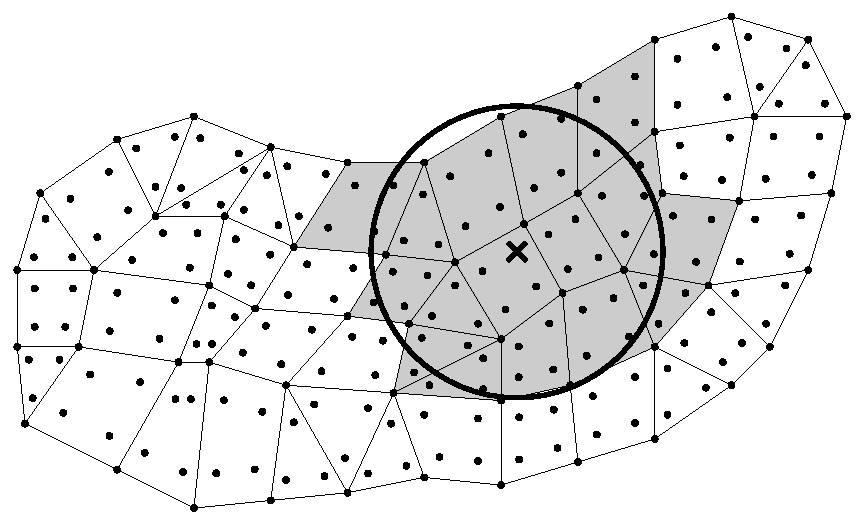
\includegraphics[width=0.4\textwidth]{pics/ApproxSQ.pdf}
    }
    \caption{Квадратурная аппроксимация области нелокального влияния}\label{fig:ApproxSQ}
\end{figure}

Матрицы СЛАУ имеют блочную структуру, поэтому введены понятия блоков матриц для уравнения теплопроводности
\[
	\widetilde{\textbf{K}}_{nm}^{e_1 e_2} (\boldsymbol{x}, \boldsymbol{y}) =
	\lambda_{ij} N_{n,i}^{e_1} (\boldsymbol{x}) N_{m,j}^{e_1} (\boldsymbol{y})
	\boldsymbol{E}_n \otimes \boldsymbol{E}_m,
\]
и уравнения равновесия
\[
	\widehat{\textbf{K}}_{nm}^{e_1 e_2} (\boldsymbol{x}, \boldsymbol{y}) = 
	C_{ijkl} N_{n,k}^{e_1} (\boldsymbol{x}) N_{m,l}^{e_2} (\boldsymbol{y}) \boldsymbol{E}_n \otimes \boldsymbol{E}_m \otimes \boldsymbol{e}_i \otimes \boldsymbol{e}_j,
\]
где $\boldsymbol{E}_n$ --- единичный вектор размерности $M$; $\boldsymbol{e}_i$ --- единичный вектор размерности 2; $i,j,k,l = \overline{1,2}$; $n,m = \overline{1,M}$; $M$ --- количество узлов в сетке $S_h$. Для общности алгоритмов обозначим блок матрицы одним символом $\textbf{K}_{nm}^{e_1 e_2}$. Тогда алгоритм ассемблирования локальной матрицы принимает форму
\begin{gather}
	\label{eq:localMatrix}
	\widehat{\textbf{K}}^L_{\mathcal{F}} =
	\sum\limits_{e \in S_h}
	\sum\limits_{n,m \in I^e}
	\sum\limits_{q \in Q^e}
	w_q \textbf{K}^{ee}_{nm} (\boldsymbol{x}_q, \boldsymbol{x}_q) J_q^e.
\end{gather}
Применим квадратурную аппроксимацию области нелокального влияния $S'(\boldsymbol{x})$, тогда алгоритм ассемблирования нелокальной матрицы представим в следующем виде
\begin{gather}
	\label{eq:NonlocalMatrix}
	\widehat{\textbf{K}}^{NL}_{\mathcal{F}} =
	\sum\limits_{e \in S_h}
	\sum\limits_{n \in I^e}
	\sum\limits_{q \in Q^e}
	w_q J_q^e
	\sum\limits_{e' \in S_h^q}
	\sum\limits_{m' \in I^{e'}}
	\sum\limits_{q' \in Q^{e'}}
	w_{q'} \varphi(\boldsymbol{x}_q, \boldsymbol{x}_{q'}) 
	\textbf{K}_{nm'}^{e e'}(\boldsymbol{x}_q, \boldsymbol{x}_{q'}) J_{q'}^{e'}.
\end{gather}
Здесь $w_q$ --- весовой множитель в квадратурном узле под номером $q$; $J_q^e$ --- якобиан преобразования из локальной системы в глобальную, аппроксимированный в квадратурном узле под номером $q$ на элементе под номером $e$.

Далее по аналогии выписаны алгоритмы ассемблирования матрицы теплообмена и векторов правой части для уравнения теплопроводности
\[
	\widehat{\textbf{K}}^{\alpha}_T =
	\sum\limits_{e \in \Gamma_h}
	\sum\limits_{n,m \in I^{e}}
	\sum\limits_{q \in Q^e}
	w_q \alpha N_n^e (\boldsymbol{x}_q) N_m^e (\boldsymbol{x}_q) J_q^e \boldsymbol{E}_n \otimes \boldsymbol{E}_m,
\]
\[
	\textbf{T}^{\alpha} =
	\sum\limits_{e \in \Gamma_h}
	\sum\limits_{n \in I^{e}}
	\sum\limits_{q \in Q^e}
	w_q \alpha N_n^e (\boldsymbol{x}_q) T_{\alpha} (\boldsymbol{x}_q) J_q^e \boldsymbol{E}_n,
\]
\[
	\textbf{Q} =
	\sum\limits_{e \in S_h}
	\sum\limits_{n \in I^e}
	\sum\limits_{q \in Q^e}
	w_q q_V (\boldsymbol{x}_q) J_q^e \boldsymbol{E}_n,
	\quad
	\textbf{F} =
	\sum\limits_{e \in \Gamma_h}
	\sum\limits_{n \in I^e}
	\sum\limits_{q \in Q^e}
	w_q f (\boldsymbol{x}_q) J_q^e \boldsymbol{E}_n,
\]
а также алгоритмы ассемблирования векторов правой части для уравнения равновесия
\[
	\widehat{\textbf{B}} =
	\sum\limits_{e \in S_h}
	\sum\limits_{n \in I^e}
	\sum\limits_{q \in Q^e}
	w_q \boldsymbol{b} (\boldsymbol{x}_q) J_q^e \boldsymbol{E}_n,
	\quad
	\widehat{\textbf{P}} = 
	\sum\limits_{e \in \Gamma_h}
	\sum\limits_{n \in I^e}
	\sum\limits_{q \in Q^e}
	w_q \boldsymbol{p} (\boldsymbol{x}_q) J_q^e \boldsymbol{E}_n,
\]
\[
	\widehat{\textbf{E}}^L = 
	\sum\limits_{e \in S_h}
	\sum\limits_{n \in I^e}
	\sum\limits_{q \in Q^e}
	w_q \nabla N_n^e (\boldsymbol{x}_q) \widehat{\mathbf{C}} \cdot \cdot \widehat{\boldsymbol{\alpha}} \Delta T (\boldsymbol{x}_q) J_q^e \boldsymbol{E}_n,
\]
\begin{multline*}
	\widehat{\textbf{E}}^{NL} = 
	\sum\limits_{e \in S_h}
	\sum\limits_{n \in I^e}
	\sum\limits_{q \in Q^e}
	w_q \nabla N_n^e (\boldsymbol{x}_q) J_q^e 
	\times \\ \times
	\sum\limits_{e' \in S_h^q}
	\sum\limits_{q' \in Q^{e'}}
	w_{q'} \varphi (\boldsymbol{x}_q, \boldsymbol{x}_{q'}) \widehat{\mathbf{C}} \cdot \cdot \widehat{\boldsymbol{\alpha}} \Delta T (\boldsymbol{x}_{q'}) J_{q'}^{e'} \boldsymbol{E}_n.
\end{multline*}
Отметим, что при аппроксимации вектора нелокального температурного линейного расширения $\widehat{\textbf{E}}^{NL}$ также был применён способ квадратурной аппроксимации области нелокального влияния $S'(\boldsymbol{x})$.

\underline{В разделе 2.4} описаны алгоритмы вычисления производных величин, таких как вектор плотности теплового потока $\boldsymbol{q}$ и тензор напряжений $\widehat{\boldsymbol{\sigma}}$. После решения СЛАУ уравнения теплопроводности (\ref{eq:ThermalSLAE}) получаем сеточную функцию температуры \textbf{T}, используя которую можем вычислить величину вектора плотности теплового потока $\boldsymbol{q}$ в квадратурном узле $q$
\[
	\boldsymbol{q}_q = 
	\left(	
	-p_1 \lambda T_m N^e_{m,k} (\boldsymbol{x}_q)
	-p_2 \sum\limits_{e' \in S_h^q} \sum\limits_{q' \in Q^{e'}} w_{q'} \lambda T_{m'} N^e_{m',k} (\boldsymbol{x}_{q'}) J^{e'}_{q'}
	\right) \boldsymbol{e}_k.
\]
Аналогично после решения СЛАУ уравнения равновесия (\ref{eq:StressSLAE}) получаем сеточную функцию вектора перемещений  $\widehat{\boldsymbol{U}}$, используя которую можем вычислить деформации $\widehat{\boldsymbol{\varepsilon}}$, а затем и напряжения
\begin{multline*}
	\widehat{\boldsymbol{\sigma}}_q =
	\Biggr(
	p_1 C_{ijkl} \left(\varepsilon_{kl} (\boldsymbol{x}_q) - \alpha_{kl} \Delta T_q \right)
	+\\+
	p_2 \sum\limits_{e' \in S_h^q} \sum\limits_{q' \in Q^{e'}} w_{q'} C_{ijkl} \left(\varepsilon_{kl} (\boldsymbol{x}_{q'}) - \alpha_{kl} \Delta T_{q'} \right) J^{e'}_{q'}
	\Biggr) \boldsymbol{e}_k \otimes \boldsymbol{e}_l.
\end{multline*}



\textbf{Третья глава} посвящена описанию реализации программного комплекса NonLocFEM.

\underline{В разделе 3.1} описана общая схема программного комплекса NonLocFEM, рассмотрена его структура, взаимосвязь модулей и их предназначение. Иллюстрация структуры в виде схемы представлена на Рис.~\ref{pic:NonLocFEMSchema}, где зависимый модуль указывает стрелкой на модуль от которого он зависит.

\begin{figure}[ht]
    \centerfloat{
        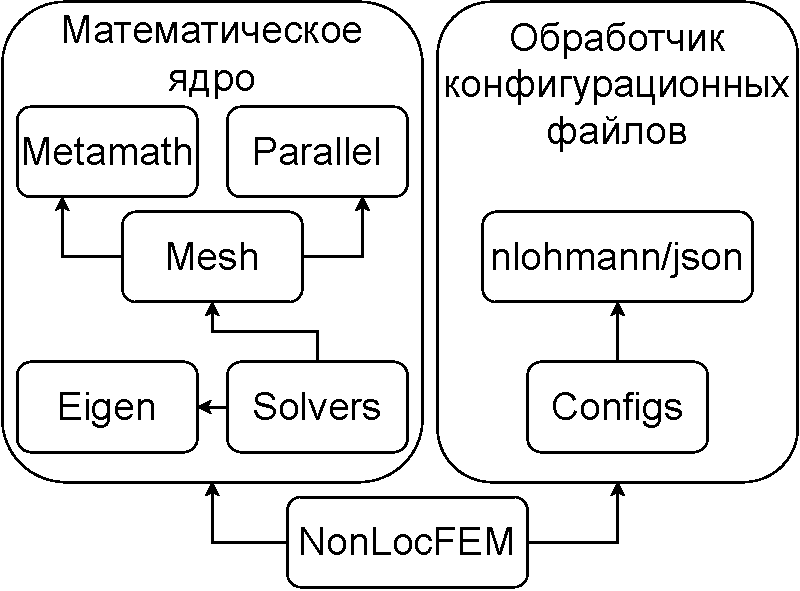
\includegraphics[width=0.4\textwidth]{pics/NonLocFEMSchema.pdf}
    }
    \caption{Структура программы NonLocFEM}\label{pic:NonLocFEMSchema}
\end{figure}

\underline{В разделе 3.2} описаны способы оптимизации и распараллеливания алгоритмов ассемблирования матриц и правых частей.

Оптимизация алгоритма ассемблирования была осуществлена путём изменения способа аппроксимации области нелокального влияния $S'(\boldsymbol{x})$. Вместо квадратурной аппроксимации предложен элементный способ аппроксимации области нелокального влияния $S'(\boldsymbol{x})$. Основным отличием данного способа от квадратурной аппроксимации является смена набора точек, по которым происходит аппроксимация области. Вместо аппроксимации относительно квадратурных узлов, поиск осуществляется относительно центров элементов. Такой подход дает возможность разделить алгоритмы заполнения матриц и интегрирования, что позволяет оптимизировать их независимо друг от друга. Иллюстрация способа представлена на Рис. \ref{fig:ApproxSE}, где крестом отмечен центр элемента, относительно которого происходит аппроксимация, точками отмечены центры элементов, кругом очерчена область нелокального влияния $S'(\boldsymbol{x})$, а серым цветом выделены элементы образующие аппроксимированную область нелокального влияния $S_h^e$.

\begin{figure}[ht]
    \centerfloat{
        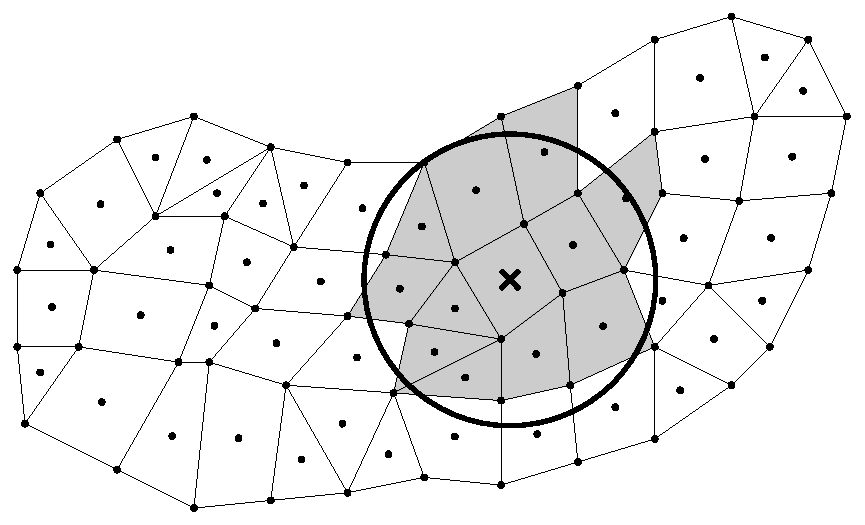
\includegraphics[width=0.4\textwidth]{pics/ApproxSE.pdf}
    }
    \caption{Элементная аппроксимация области нелокального влияния}\label{fig:ApproxSE}
\end{figure}

Распараллеливание алгоритмов выполнено посредством изменения порядка суммирования по элементам и проекционным узлам в алгоритмах ассемблирования (\ref{eq:localMatrix}) и (\ref{eq:NonlocalMatrix}), но чтобы это сделать необходимо для каждого узла составить список элементов $E^n$, которым он принадлежит. В результате алгоритмы принимают вид
\begin{gather*}
	\widehat{\textbf{K}}^L_{\mathcal{F}} =
	\sum\limits_{n \in S_h}
	\sum\limits_{e \in E^n}
	\sum\limits_{m \in I^e}
	\sum\limits_{q \in Q^e}
	w_q \textbf{K}^{ee}_{nm} (\boldsymbol{x}_q, \boldsymbol{x}_q) J_q^e,
\end{gather*}
\begin{gather}
	\label{eq:ParallelNonlocalMatrix}
	\widehat{\textbf{K}}^{NL}_{\mathcal{F}} =
	\sum\limits_{n \in S_h}
	\sum\limits_{e \in E^n}
	\sum\limits_{e' \in S_h^e}
	\sum\limits_{m \in I^{e'}}
	\sum\limits_{q \in Q^e}
	w_q J_q^e
	\sum\limits_{q' \in Q^{e'}}
	w_{q'} \varphi(\boldsymbol{x}_q, \boldsymbol{x}_{q'}) 
	\textbf{K}_{nm}^{e e'}(\boldsymbol{x}_q, \boldsymbol{x}_{q'}) J_{q'}^{e'}.
\end{gather}
При таком подходе сборка матриц происходит построчно, что открывает широкие возможности для распараллеливания. Каждая строка может быть обработана независимо в отдельном потоке исполнения, а вычисление группы строк легко распределить между процессами.

\underline{В разделе 3.3} приведено описание алгоритма аппроксимации области нелокального влияния $S'(\boldsymbol{x})$ на основе k-d дерева. Суть алгоритма заключается в дроблении области на равномерные ячейки, где длина стороны ячейки равна радиусу поиска. Затем каждой ячейке присваивают узлы, которые находятся в её области, после чего поиск соседних узлов относительно текущего рассматриваемого узла сужается до ячейки, в которой он находится, и смежных с ней ячейкам, где уже используется алгоритм линейного поиска. Сложность итогового алгоритма можно оценить как $O(N \log N)$, где $N$ --- количество узлов.

\underline{В разделе 3.4} описано семейство базисных функций квадратичного серендипового (8-узлового) элемента. Данное семейство базисов обладает свободным параметром $s$, вариация которого приводит к изменению числа обусловленности матриц теплопроводности и жёсткости. Путём минимизации следа матрицы была предложена оценка, согласно которой числа обсуловленности должны быть минимальными при $s = 2/9$.

\textbf{Четвёртая глава} посвящена результатам расчётов с проведением сравнительного анализа представленных в работе моделей.

\underline{В разделе 4.1} описана стратегия исследования, принятые гипотезы, а также проведено обезразмеривание моделей теплопроводности и термоупругости. Далее все безразмерные параметры и величины будем обозначать теми же символами, что и в исходных уравнениях, но с чертой над символом.

\underline{В разделе 4.2} представлены основные особенности решений. Сравнения локальной и нелокальной теорий при различных параметрах моделей проводились на области $S = \left\{ \overline{\boldsymbol{x}} \ | \ -0.5 \leqslant \overline{x}_1, \overline{x}_2 \leqslant 0.5 \right\}$, где были решены задача о прохождении сквозь неё теплового потока и задача об одноосном растяжении. Было установлено, что решения в нелокальном случае обладают кромочным эффектом, который характеризуется увеличенными значениями температуры и перемещений на кромках, где заданы нагружения. Также было установлено появление ненулевых полей компоненты вектора плотности теплового потока $\overline{q}_2$ и касательной компоненты тензора напряжений $\overline{\sigma}_{12}$. Установлены зависимости влияния основных параметров модели на распределения полей решений.

\underline{В разделе 4.3} проведён сравнительный анализ полиномиального (\ref{eq:Polynomial}) и экспоненциального (\ref{eq:Exponential}) семейств функций нелокального влияния. Показано, что оба семейства имеют одинаковое поведение при вариации параметров обозначенных одними и теми же символами. В заключении раздела был сделан вывод, что качественных различий между решениями при различных функциях нелокального влияния нет и выбор функции влияет лишь на величину отклонений, поэтому дальнейшие исследования были проведены с использованием квадратичной параболы, то есть была выбрана функция полиномиального семейства (\ref{eq:Polynomial}) с параметрами $n = 2$, $p = 2$ и $q = 1$.

\underline{В разделе 4.4} изучены принципы стабильности теплового потока и Сен-Венана. Для их изучения была рассмотрена прямоугольная область $S = \left\{ \boldsymbol{x} | -5 \leqslant x_1 \leqslant 5, -0.5 \leqslant x_2 \leqslant 0.5 \right\}$, на которой при изучении принципа стабильности тепловых потоков для уравнения теплопроводности были поставлены следующие граничные условия Неймана и, для единственности решения, дополнительное интегральное условие:
\begin{gather*}
	\boldsymbol{n} \cdot \overline{\boldsymbol{q}} |_{\overline{x}_1 = -5} = f(\overline{x}_2),
	\quad
	\boldsymbol{n} \cdot \overline{\boldsymbol{q}} |_{\overline{x}_1 = 5} = -f(\overline{x}_2),
	\quad
	\iint\limits_S T dS = 0.
\end{gather*}
Аналогично при изучении принципа Сен-Венана были поставлены граничные и геометрические условия для уравнения равновесия:
\begin{gather*}
	n_j \overline{\sigma}_{j1} |_{\overline{x}_1 = -5} = -f(\overline{x}_2),
	\quad
	n_j \overline{\sigma}_{j1} |_{\overline{x}_1 = 5} = f(\overline{x}_2),
	\quad
	\overline{u}_1 |_{\overline{x}_1 = 0} = 0,
	\quad
	\overline{u}_2 |_{\overline{x}_2 = 0} = 0.
\end{gather*}
Здесь $f$ --- нормированная функция. Исследованы три варианта нагружения: равномерное и два треугольных, развёрнутых в разные стороны, которые определены при помощи следующих функций
\begin{gather*}
	f_1 (x) = 1,
	\quad
	f_2 (x) = 2 - 4 |x|,
	\quad
	f_3 (x) = 4 |x|.
\end{gather*}

Анализ решений показал, что при различных нагружениях первая компонента вектора плотности теплового потока $\overline{q}_1$ и компонента тензора напряжений $\overline{\sigma}_{11}$ сливаются в общую поверхность вдали от точек приложения нагружений. В классическом случае решения сливаются в плоскость, равную 1, нелокальные образуют более сложную поверхность. На Рис. \ref{fig:SaintVenantVariation} представлены распределения $\overline{q}_1$ и $\overline{\sigma}_{11}$ в сечении $\overline{x}_1 = 0$, где из-за равенства обозначены по оси ординат общим символом $\mathcal{S}$. Нелокальные решения имеют кромочный эффект, характеризующийся снижением рассматриваемой величины на свободных от условий границах и её увеличением внутри области. При этом увеличение радиуса нелокальности $\overline{r}$ приводит к увеличению размаха кромочного эффекта, а уменьшение параметра $p_1$ --- к увеличению отклонений.

\begin{figure}[ht] \centering
	\begin{tabular}{cc}
		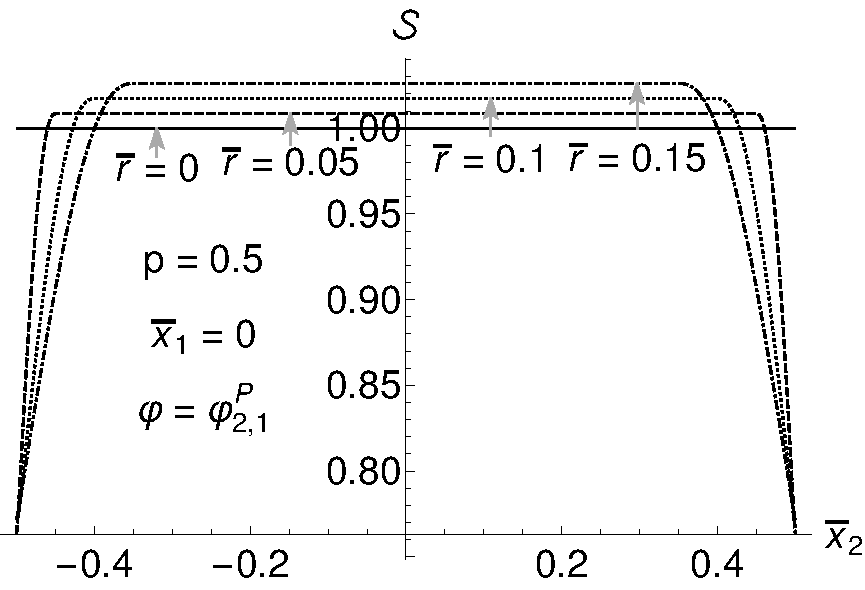
\includegraphics[width=0.4\linewidth]{pics/HeatFluxStabilityVariationR.pdf} &
		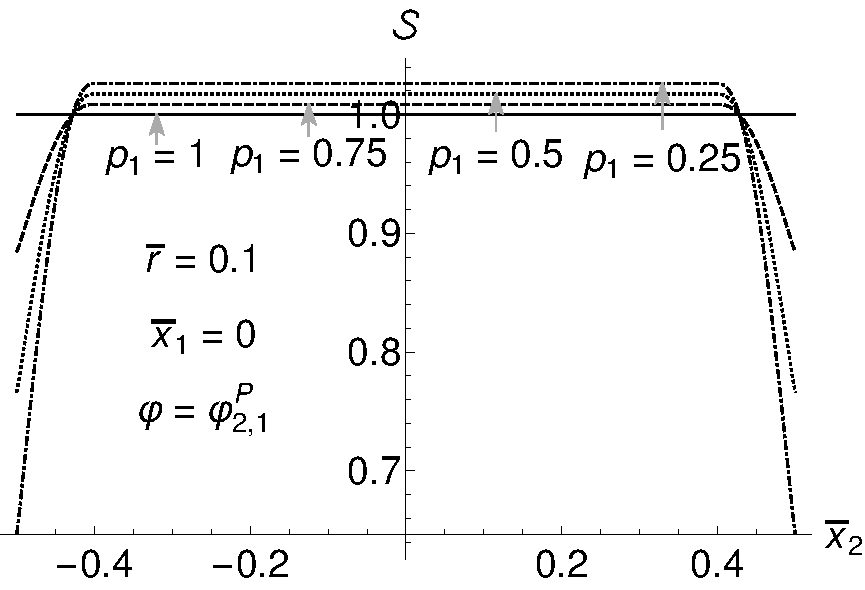
\includegraphics[width=0.4\linewidth]{pics/HeatFluxStabilityVariationP1.pdf} \\
		а) & б)
	\end{tabular}
    \caption{Распределение компоненты теплового потока $\overline{q}_1$ и компоненты тензора напряжений $\overline{\sigma}_{11}$ в сечении $\overline{x}_1 = 0$ при вариации $\overline{r}$ (а) и $p_1$ (б)}
    \label{fig:SaintVenantVariation}
\end{figure}

Во всех сечениях равнодействующие компоненты теплового потока $\overline{q}_1$ и напряжения $\overline{\sigma}_{11}$ сохраняются и равны приложенным нагружениям:
\begin{gather*}
	\int\limits_{-0.5}^{0.5} \overline{q}_1 d\overline{x}_2 = 
	\int\limits_{-0.5}^{0.5} f_i (\overline{x}_2) d\overline{x}_2,
	\quad
	\int\limits_{-0.5}^{0.5} \overline{\sigma}_{11} d\overline{x}_2 = 
	\int\limits_{-0.5}^{0.5} f_i (\overline{x}_2) d\overline{x}_2,
	\quad	
	i = \overline{1,3}.
\end{gather*}
Это свидетельствует о выполнении принципов стабильности теплового потока и Сен-Венана, а также сохранении балансных соотношений.

\underline{В разделе 4.5} решена задача о растяжении пластины со ступенчатым переходом. Здесь к Т-образной области были приложены граничные и геометрические условия
\begin{gather*}
	n_j \overline{\sigma}_{j2} |_{\overline{x}_2 = 0} = -1,
	\quad
	\overline{u}_2 |_{\overline{x}_2 = 1} = 0,
	\quad
	\overline{u}_1 |_{\overline{x}_1 = 0.5} = 0.
\end{gather*}

%\begin{figure}[ht]
%    \centering
%    \begin{tabular}{ccc}
%	    	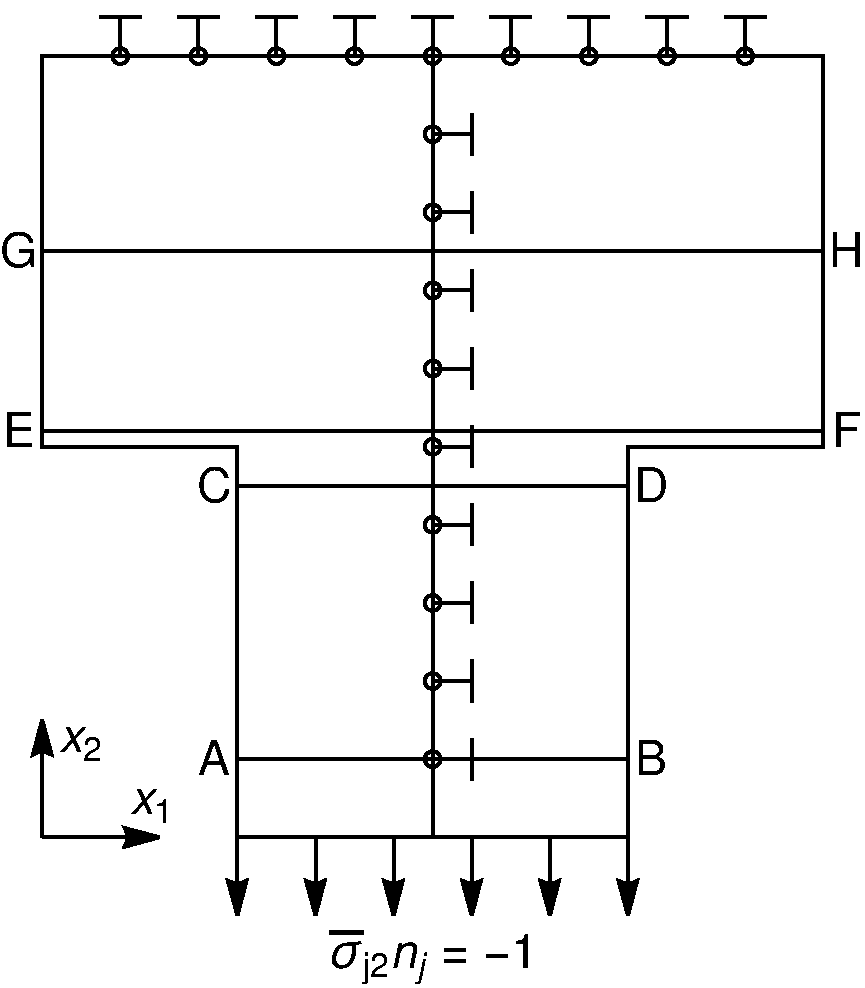
\includegraphics[width=0.24\textwidth]{pics/TArea.pdf} &
%        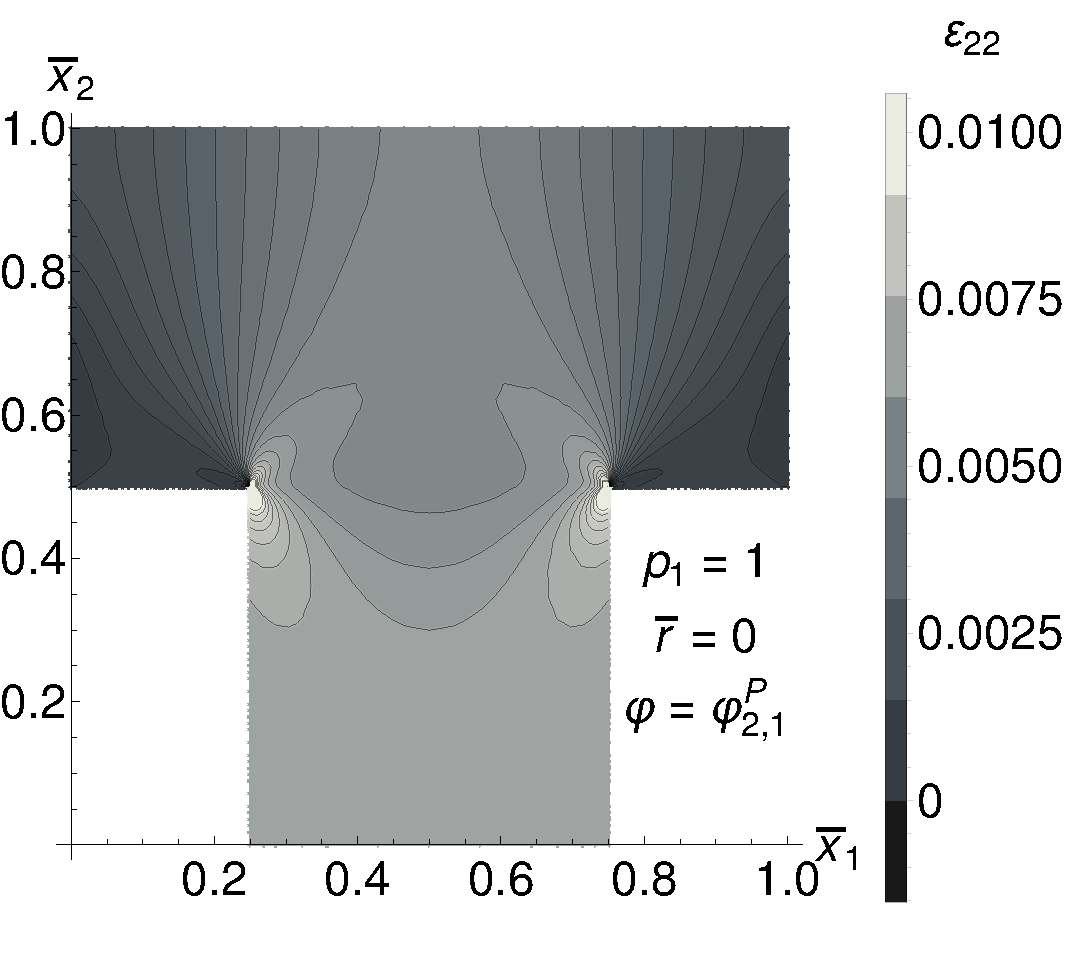
\includegraphics[width=0.33\textwidth]{pics/TEpsR0.pdf} &
%        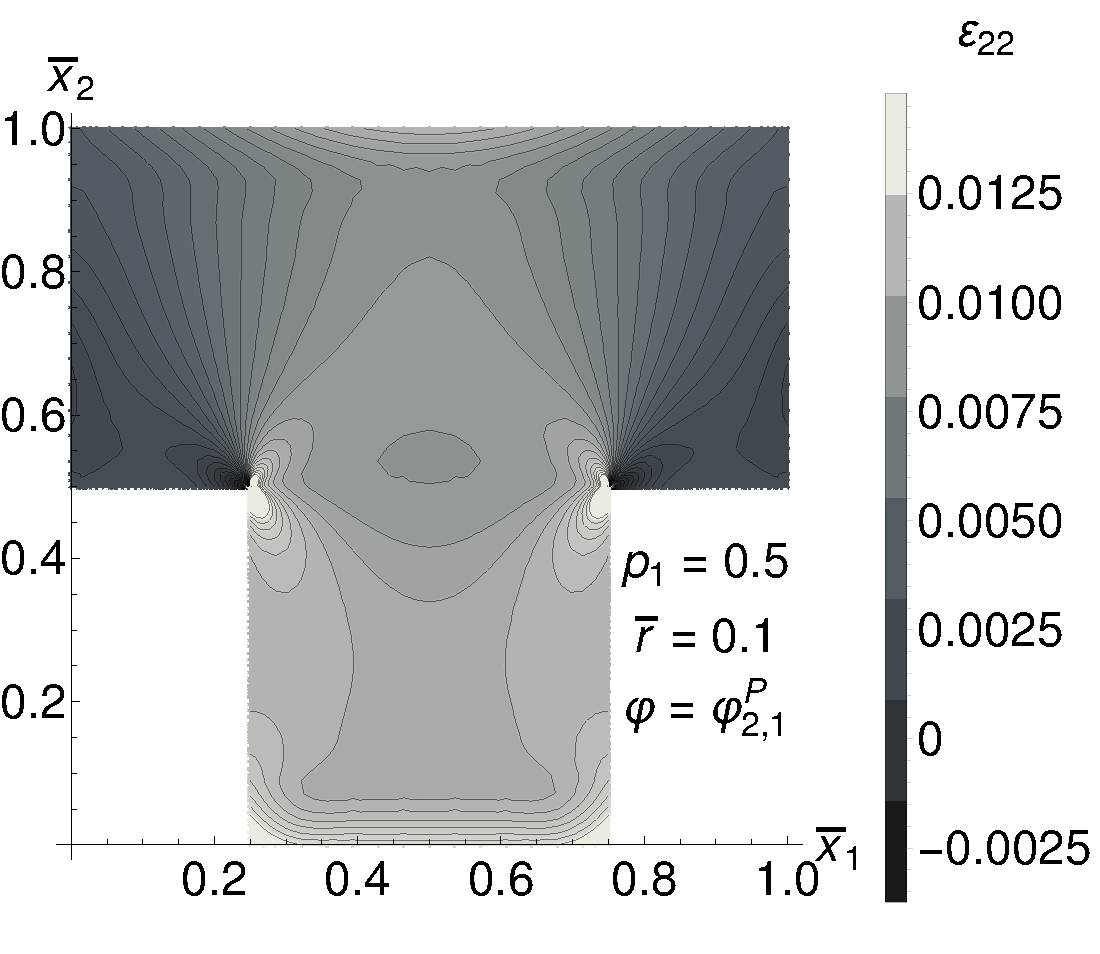
\includegraphics[width=0.33\textwidth]{pics/TEpsR01.pdf} \\
%        а) & б) & в)
%    \end{tabular}
%    \caption{Т-образная область с приложенной нагрузкой (а) и распределение компоненты тензора деформации $\varepsilon_{22}$ при $p_1 = 0.5$ (б) --- $\overline{r} = 0$ и (в) --- $\overline{r} = 0.1$}
%    \label{fig:TEpsilon}
%\end{figure}

Проведённый анализ решений показал, что в нелокальном случае решения обладают особенностями в углах между верхней и нижней частями области, где в смежной с концентратором верхней части области наблюдаем области с отрицательными значениями деформации. Также отметим, что в нелокальном случае линии уровней обладают изломом вблизи верхней границы, а вблизи с кромкой, к которой приложена нагрузка, появляются дополнительные линии уровней.

\underline{В разделе 4.6} решена задача Кирша с обобщением на эллиптические вырезы (Рис. \ref{fig:KirshProblem}). Были поставлены следующие граничные и геометрические условия
\begin{gather*}
	n_j \overline{\sigma}_{j1} |_{\overline{x}_1 = -1} = -1,
	\quad
	n_j \overline{\sigma}_{j1} |_{\overline{x}_1 = 1} = 1,
	\quad
	\overline{u}_1 |_{\overline{x}_1 = 0} = 0,
	\quad
	\overline{u}_2 |_{\overline{x}_2 = 0} = 0.
\end{gather*}

\begin{figure}[ht]
    \centerfloat{
        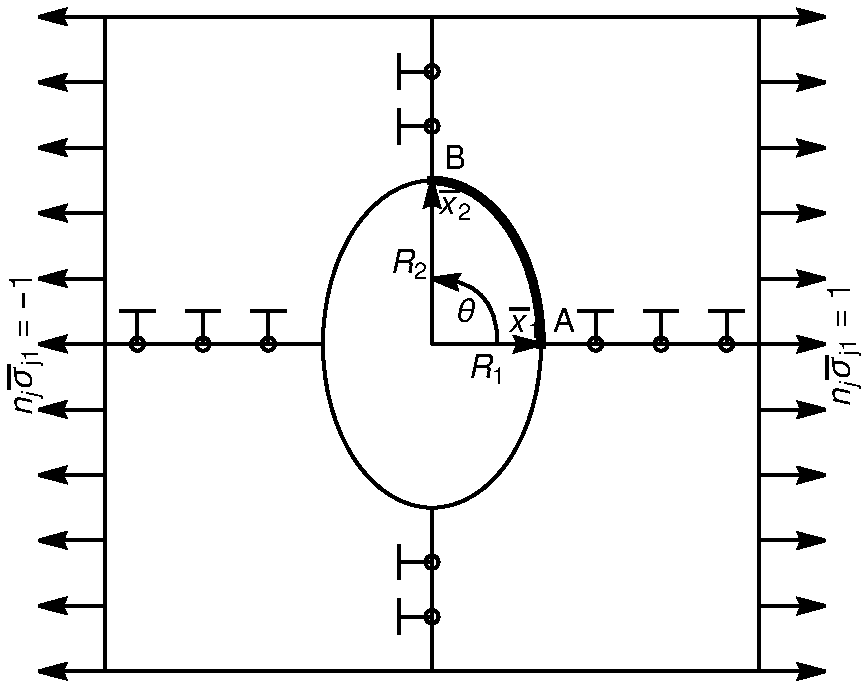
\includegraphics[width=0.45\textwidth]{pics/EllipseStress.pdf}
    }
    \caption{Постановка задачи Кирша}
    \label{fig:KirshProblem}
\end{figure}

Известно, что максимальные напряжения находятся в верхней и нижней точках выреза, а их величина в классическом случае подчиняется следующей закономерности
\begin{gather*}
	\overline{\sigma}_{11}^{\max} = \left( 1 + 2 \rho \right) \sigma_0,
\end{gather*}
где $\sigma_0$ --- равнодействующая величина прикладываемого нагружения, а $\rho = R_2 / R_1$. В диссертации показано, что в нелокальном случае появляется дополнительный множитель $\kappa$, который зависит от весового параметра модели $p_1$. В этом случае
 \begin{gather*}
	\overline{\sigma}_{11}^{\max} = \kappa \left( 1 + 2 \rho \right) \sigma_0.
\end{gather*}
Такая зависимость не имеет строго теоретического подтверждения и получена эвристически, однако, она может быть полезна для оценок в практических расчётах. Дополнительно отметим лишь, что параметра $\kappa$ уменьшается вместе с параметром $p_1$, то есть максимальный уровень напряжения в нелокальных постановках ниже, чем в классической.

\underline{В разделе 4.7} решена задача термоупругости в областях с эллиптическими вырезами (Рис. \ref{fig:ThermalKirshProblem}). Для этого были поставлены следующие граничные и интегральные условия:
\begin{gather*}
	\boldsymbol{n} \cdot \overline{\boldsymbol{q}}|_{\overline{x}_1 = -1} = 1,
	\quad
	\boldsymbol{n} \cdot \overline{\boldsymbol{q}}|_{\overline{x}_1 = 1} = -1,
	\quad
	\overline{u}_2 |_{\overline{x}_1 = 0} = 0,
	\\
	\iint\limits_S \overline{T} dS = 0,
	\quad
	\iint\limits_S \overline{u}_1 dS = 0.
\end{gather*}
Такая постановка удобна тем, что позволяет качественно изучить поведение температурных напряжений без появления дополнительных напряжений со стороны возможных концентраторов, обусловленных граничными или геометрическими условиями.

\begin{figure}[ht]
    \centerfloat{
        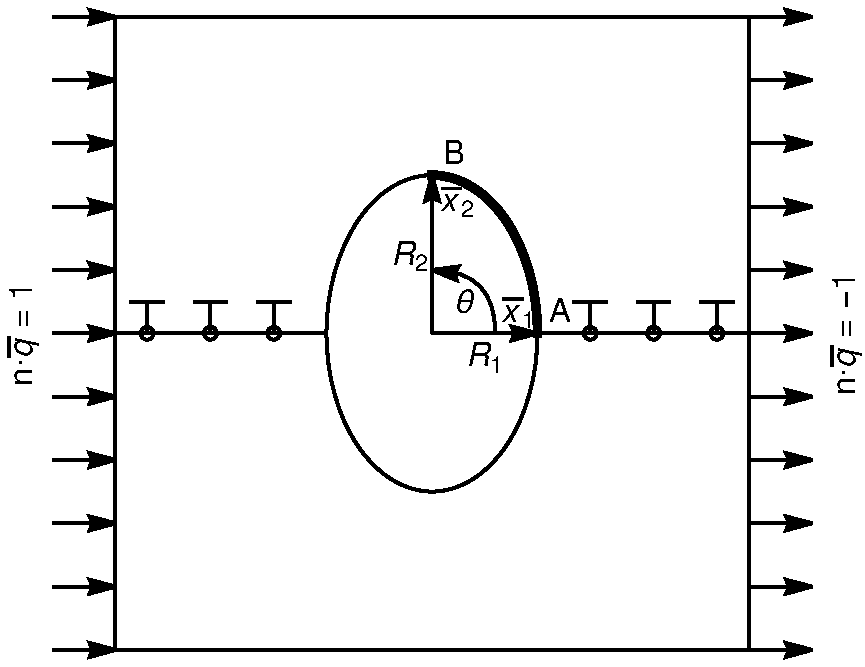
\includegraphics[width=0.45\textwidth]{pics/EllipseThermal.pdf}
    }
    \caption{Тепловые нагружения в области с эллиптическим вырезом}
    \label{fig:ThermalKirshProblem}
\end{figure}

Здесь, аналогично задаче Кирша, максимальные значения компоненты вектора плотности теплового потока $\overline{q}_1$ находятся в верхней и нижней точках выреза и они подчиняются зависимости
\begin{gather*}
	\overline{q}_1^{\max} = (1 + \rho) q_o.
\end{gather*}
В нелокальном случае это значение уменьшается, но установить такую же прочную связь, как и в случае с уравнением равновесия, не удаётся.

Решения относительно напряжений обладают симметрией, причём относительно верхней и нижней частей области решения чётные, а относительно правой и левой нечётные. Напряжения в нелокальном случае, как и во всех предыдущих случаях, становятся ниже, чем в классическом случае (Рис.~\ref{fig:ThermalKirshP1Variation}).

\begin{figure}[ht] \centering
	\begin{tabular}{cc}
		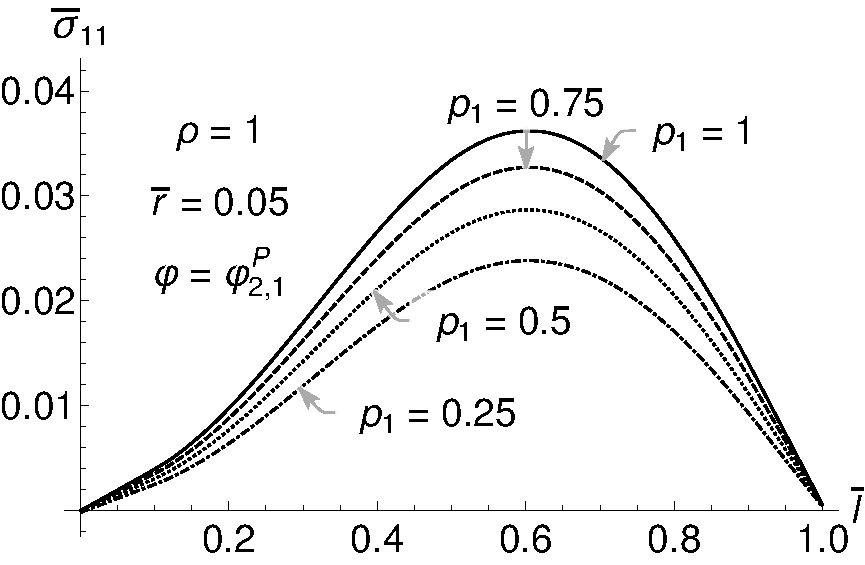
\includegraphics[width=0.38\linewidth]{pics/ThermalKirshSigma11VariationP1.pdf} &
		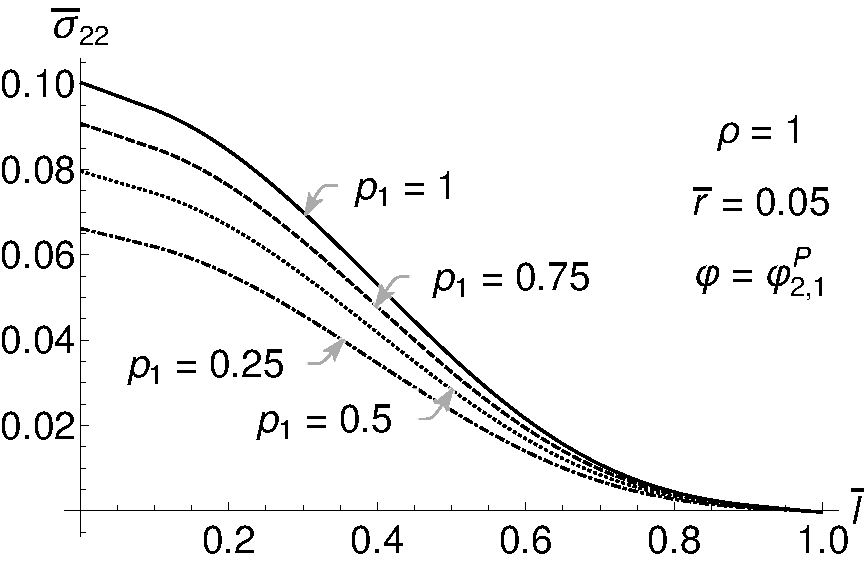
\includegraphics[width=0.38\linewidth]{pics/ThermalKirshSigma22VariationP1.pdf} \\
		а) & б)
	\end{tabular}
    \caption{Распределение напряжения $\overline{\sigma}_{11}$ (a) и $\overline{\sigma}_{22}$ (б) на кромке AB при вариации весового параметра $p_1$}
    \label{fig:ThermalKirshP1Variation}
\end{figure}

\textbf{Пятая глава} посвящена исследованию эффективности реализации программного комплекса NonLocFEM.

\underline{В разделе 5.1} проведено исследование масштабируемости алгоритмов ассемблирования матриц теплопроводности и жёсткости (\ref{eq:ParallelNonlocalMatrix}). На Рис.~\ref{fig:OMPParallelization} представлены столбцовые диаграммы эффективности ускорения на 18 ядерном процессоре Intel Core i9
10980XE при использовании технологии OpenMP, где ускорение времени ассемблирования матриц в нелокальных постановках достигает 14 раз при использовании всех ядер процессора.

\begin{figure}[ht] \centering
	\begin{tabular}{cc}
		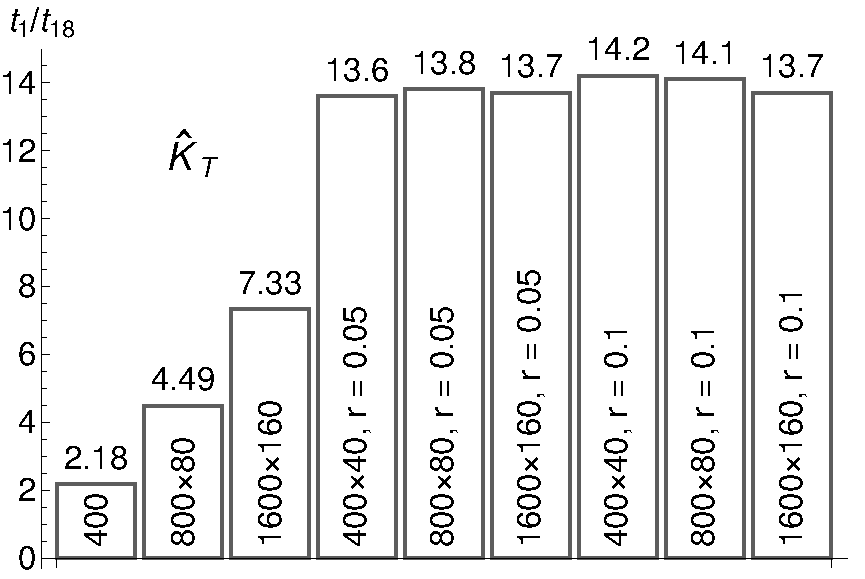
\includegraphics[width=0.38\linewidth]{pics/OMPThermal.pdf} &
		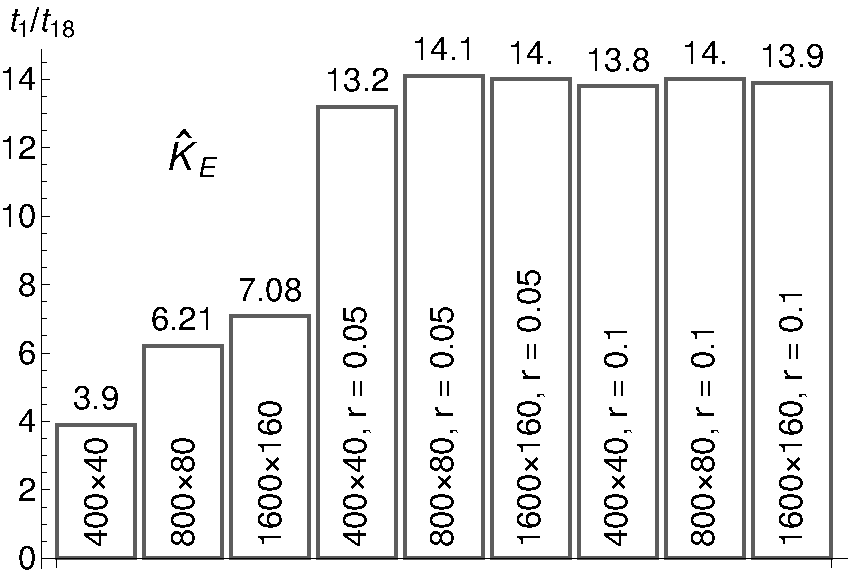
\includegraphics[width=0.38\linewidth]{pics/OMPMechanical.pdf} \\
		а) & б)
	\end{tabular}
    \caption{Эффективность распараллеливания алгоритма сборки матриц (а)~теплопроводности и (б)~жёсткости при использовании OpenMP}
    \label{fig:OMPParallelization}
\end{figure}

Также в этом разделе был изучен вопрос эффективности алгоритмов балансировки данных между процессами при использовании технологии MPI. Показано, что использование этого алгоритма даёт равномерное распределение данных между процессами.

\underline{В разделе 5.2} проведено исследование скорости сходимости метода сопряжённых градиентов при решении СЛАУ (\ref{eq:StressSLAE}). Была поставлена задача равновесия на сетке $S_h$, состоящей из $1000 \times 100$ элементов, после чего была вычислена связь между параметром базиса $s$ и весовым параметром модели $p_1$ с числом обусловленности матрицы жёсткости (Рис.~\ref{fig:MechanicalCondAndIter}). Графики сходимости метода сопряжённых градиентов хорошо коррелируют с графиками числа обусловленности, кроме того они демонстрируют корректность оценки, полученной в разделе 3.4, согласно которой минимум числа обусловленности находится в окрестностях точки $s = 2/9$.

\begin{figure}[ht] \centering
	\begin{tabular}{cc}
		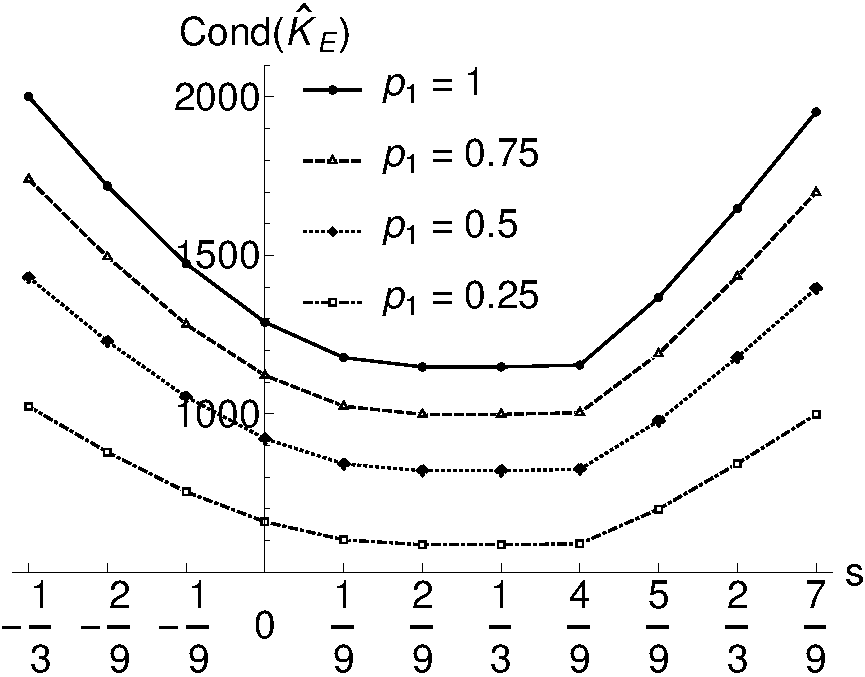
\includegraphics[width=0.38\linewidth]{pics/MechanicalCond.pdf} &
		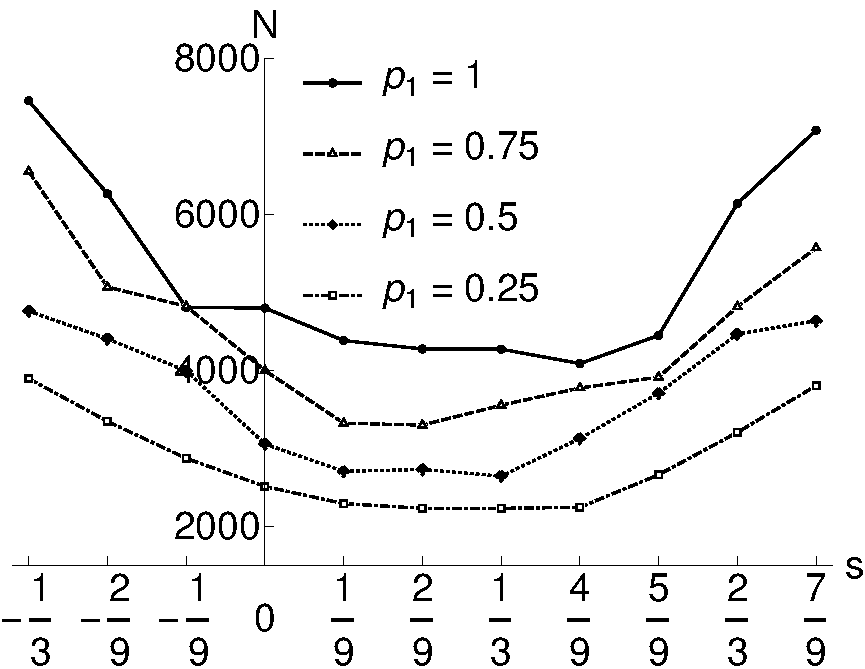
\includegraphics[width=0.38\linewidth]{pics/MechanicalIter.pdf} \\
		а) & б)
	\end{tabular}
    \caption{Зависимость числа обусловленности (а) и количества итераций $N$ (б) для матрицы жёсткости $\widehat{\textbf{K}}_E$ от параметров $s$ и $p_1$ при $r = 0.1$}
    \label{fig:MechanicalCondAndIter}
\end{figure}

%\begin{figure}[ht]
%    \begin{minipage}[b][][b]{0.4\linewidth}\centering
%        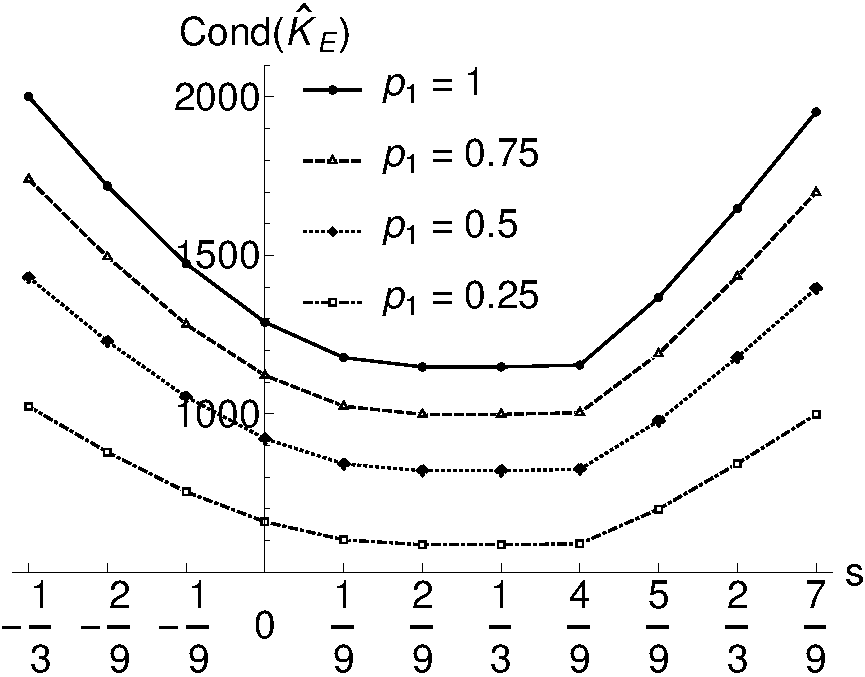
\includegraphics[width=\linewidth]{pics/MechanicalCond.pdf} \\ а)
%    \end{minipage}
%    \hfill
%    \begin{minipage}[b][][b]{0.4\linewidth}\centering
%        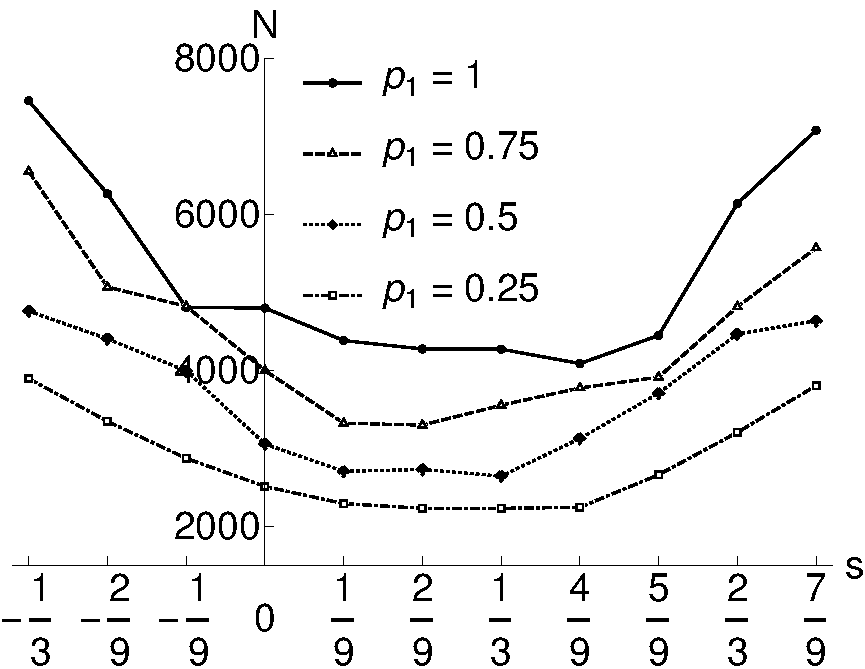
\includegraphics[width=\linewidth]{pics/MechanicalIter.pdf} \\ б)
%    \end{minipage}
%    \caption{Зависимость (а) числа обусловленности и (б) количества итераций $N$ для матрицы жёсткости $\widehat{\textbf{K}}_E$ от параметров $s$ и $p_1$ при $r = 0.1$}
%    \label{fig:MechanicalCondAndIter}
%\end{figure}

\underline{В разделе 5.3} исследована возможность предобуславливания СЛАУ, полученных в нелокальных задачах, при помощи неполного разложения Холецкого локальной матрицы. Результаты показали, что ускорение сходимости  метода сопряжённых градиентов достигает 2.5 раз. При этом объём затрачиваемой оперативной памяти, который занимает локальная матрица, достаточно мал по сравнению с нелокальной матрицей, что делает такой способ предобуславливания экономичным с точки зрения использования вычислительных ресурсов.

%Можно сослаться на свои работы в автореферате. Для этого в файле
%\verb!Synopsis/setup.tex! необходимо присвоить положительное значение
%счётчику \verb!\setcounter{usefootcite}{1}!. В таком случае ссылки на
%работы других авторов будут подстрочными.
%Изложенные в третьей главе результаты опубликованы в~\cite{vakbib1, vakbib2}.
%Использование подстрочных ссылок внутри таблиц может вызывать проблемы.

\FloatBarrier
\pdfbookmark{Заключение}{conclusion}                                  % Закладка pdf
%\textbf{В заключении} приведены основные результаты работы, которые заключаются в следующем:
\begin{center}
	\textbf{ОСНОВНЫЕ РЕЗУЛЬТАТЫ ДИССЕРТАЦИОННОЙ РАБОТЫ}
\end{center}
%% Согласно ГОСТ Р 7.0.11-2011:
%% 5.3.3 В заключении диссертации излагают итоги выполненного исследования, рекомендации, перспективы дальнейшей разработки темы.
%% 9.2.3 В заключении автореферата диссертации излагают итоги данного исследования, рекомендации и перспективы дальнейшей разработки темы.
\begin{enumerate}
	\item Рассмотрена иерархия моделей нелокальной теплопроводности и термоупругости, предложено и проанализировано два семейства возможных функций нелокального влияния, заданных на областях, ограниченных кривыми Ламэ.
	
	\item Разработан численный алгоритм решения интегро-дифференциальных уравнений на основе метода конечных элементов, проведена работа над его оптимизацией и подготовкой к использованию в параллельной среде вычислений.
	
	\item Разработан собственный программный комплекс NonLocFEM, в рамках которого реализованы все предложенные алгоритмы; параллельные реализации алгоритмов задействуют технологии параллельного программирования OpenMP и MPI, все исследования и расчёты проведены в рамках программного комплекса.
	
	\item Проведён качественный анализ сравнения классических теорий теплопроводности и термоупругости с их нелокальными постановками, полученные результаты свидетельствуют о снижении роли концентраторов в распределениях полей напряжений и плотности теплового потока и в возникновении кромочных эффектов на свободных от граничных условий границах, а также определены основные зависимости отклонений нелокальных решений относительно классическим путём вариации параметров модели.
	
	\item Исследован вопрос сходимости итерационных методов решения СЛАУ применительно к задачам в нелокальных постановках, предложены способы ускорения сходимости с применением альтернативных базисов конечных элементов и предобуславливателей.
\end{enumerate}


\pdfbookmark{Литература}{bibliography}                                % Закладка pdf
%При использовании пакета \verb!biblatex! список публикаций автора по теме
%диссертации формируется в разделе <<\publications>>\ файла
%\verb!common/characteristic.tex!  при помощи команды \verb!\nocite!

\begin{comment}
\ifdefmacro{\microtypesetup}{\microtypesetup{protrusion=false}}{} % не рекомендуется применять пакет микротипографики к автоматически генерируемому списку литературы
\urlstyle{rm}                               % ссылки URL обычным шрифтом
\ifnumequal{\value{bibliosel}}{0}{% Встроенная реализация с загрузкой файла через движок bibtex8
    \renewcommand{\bibname}{\large \bibtitleauthor}
    \nocite{*}
    \insertbiblioauthor           % Подключаем Bib-базы
    %\insertbiblioexternal   % !!! bibtex не умеет работать с несколькими библиографиями !!!
}{% Реализация пакетом biblatex через движок biber
    % Цитирования.
    %  * Порядок перечисления определяет порядок в библиографии (только внутри подраздела, если `\insertbiblioauthorgrouped`).
    %  * Если не соблюдать порядок "как для \printbibliography", нумерация в `\insertbiblioauthor` будет кривой.
    %  * Если цитировать каждый источник отдельной командой --- найти некоторые ошибки будет проще.
    %
    %% authorvak
    \nocite{vakbib1}%
    \nocite{vakbib2}%
    %
    %% authorwos
    \nocite{wosbib1}%
    %
    %% authorscopus
    \nocite{scbib1}%
    %
    %% authorpathent
    \nocite{patbib1}%
    %
    %% authorprogram
    \nocite{progbib1}%
    %
    %% authorconf
    \nocite{confbib1}%
    \nocite{confbib2}%
    %
    %% authorother
    \nocite{bib1}%
    \nocite{bib2}%

    \ifnumgreater{\value{usefootcite}}{0}{
        \begin{refcontext}[labelprefix={}]
            \ifnum \value{bibgrouped}>0
                \insertbiblioauthorgrouped    % Вывод всех работ автора, сгруппированных по источникам
            \else
                \insertbiblioauthor      % Вывод всех работ автора
            \fi
        \end{refcontext}
    }{
        \ifnum \totvalue{citeexternal}>0
            \begin{refcontext}[labelprefix=A]
                \ifnum \value{bibgrouped}>0
                    \insertbiblioauthorgrouped    % Вывод всех работ автора, сгруппированных по источникам
                \else
                    \insertbiblioauthor      % Вывод всех работ автора
                \fi
            \end{refcontext}
        \else
            \ifnum \value{bibgrouped}>0
                \insertbiblioauthorgrouped    % Вывод всех работ автора, сгруппированных по источникам
            \else
                \insertbiblioauthor      % Вывод всех работ автора
            \fi
        \fi
        %\insertbiblioauthorimportant  % Вывод наиболее значимых работ автора (определяется в файле characteristic во второй section)
        \begin{refcontext}[labelprefix={}]
            %\insertbiblioexternal            % Вывод списка литературы, на которую ссылались в тексте автореферата
        \end{refcontext}
        % Невидимый библиографический список для подсчёта количества внешних публикаций
        % Используется, чтобы убрать приставку "А" у работ автора, если в автореферате нет
        % цитирований внешних источников.
        \printbibliography[heading=nobibheading, section=0, env=countexternal, keyword=biblioexternal, resetnumbers=true]%
    }
}
\ifdefmacro{\microtypesetup}{\microtypesetup{protrusion=true}}{}
\urlstyle{tt}                               % возвращаем установки шрифта ссылок URL
\end{comment}

\textbf{Основные результаты диссертации отражены в работах}

1. Кувыркин Г. Н., Соколов А. А. Принцип Сен-Венана в задачах нело­кальной теории упругости // Вестник МГТУ им. Н.Э. Баумана. Сер. Естественные науки. 2023. Т. 109. № 4. С. 4—17. (0.55 п.л./0.3 п.л.)

2. Кувыркин Г. Н., Соколов А. А. Решение задачи о напряженно-дефо\-рмиро­ванном состоянии пластины с эллиптическим вырезом при механических и температурных нагружениях в нелокальной постановке // Прикладная механика и техническая физика. 2024. No 4. С. 193—203. (0.4 п.л./0.2 п.л.)

3. Свидетельство о гос. регистрации программы для ЭВМ. NonLocFEM / А. А. Соколов; А. А. Соколов, И. Ю. Савельева. №2021661966; заявл. 20.07.2021; опубл. 22.09.2022, РД040930 (Рос. Федерация).

4. Kuvyrkin G. N., Savelyeva I. Y., Sokolov A. A. 2D nonlocal elasticity: In vestigation of stress and strain fields in complex shape regions // Z Angew Math Mech. 2023. Vol. 103. (0.6 п.л./0.3 п.л.)

5. Kuvyrkin G. N., Savelyeva I. Y., Sokolov A. A. Features of the software implementation of the numerical solution of stationary heat equation taking into account the effects of nonlocal finite element method // Journal of Physics: Conference Series. 2020. Vol. 1479. № 1. (0.4 п.л./0.2 п.л.)

6. Mathematical modeling of insulating coating of thermal conductivity in cluding body`s own radiation and non-local spatial effects / G. N. Kuvyrkin [et al.] // Journal of Physics: Conference Series. 2024. Vol. 2817. № 1. P. 12—28. (0.35 п.л./0.1 п.л.)